% !TeX spellcheck = en_US
\documentclass[12pt]{article}

% Language setting
\usepackage[TU]{fontenc}
\usepackage[ukrainian]{babel}
\usepackage{fontspec}
\setmainfont[
  Path = ./assets/fonts/,
  Extension = .ttf,
  UprightFont = *-Regular,
  ItalicFont = *-Italic,
  BoldFont = *-Bold,
  BoldItalicFont = *-BoldItalic]{LiberationSerif}

\def\sections{sections/translated/ua}
\def\lang_header_adjustment{0px}

\newcommand{\version}{
  Версія 1.2
}

\newcommand{\intro}{
  Цей проект розвивається спільнотою і має власний \href{https://github.com/Heegu-sama/Homm3BG}{репрозиторій на GitHub}.
    Вітаються будь-які зміни та виправлення .
  Якщо ви просто хочете залишити відгук, будь ласка, робіть це в оригінальній  \href{https://boardgamegeek.com/thread/3235221/rule-book-rewrite-project}{темі на BoardGameGeek}.
}
\newcommand{\pageshorthand}{с.}

\newcommand{\heegusquote}{
  \textit{На жаль, ця гра недопрацьована.
    Очевидно, що у фан-сервіс вкладено багато любові, особливо коли мова йде про візуальну складову, але геймплей не дуже вдалий.
    У вас будуть моменти екстазу, коли ви будете знищувати слабких ворогів, але так само багато розчарувань через погані кидки кісток і витягнуті карти.
    Це дуже "америтрешний" стиль гри, якого, мабуть, не очікували фанати відеоігри.
    Я не буду звинувачувати вас, якщо ви очікували зіграти в полегшену версію Mage Knight, але ця гра просто відходить далеко в протилежний бік від стратегічного мислення Mage Knight.
    \\
    Це гра, в якій, в її нинішньому стані, фанати повинні перетворити її на щось більше.
    Я сподіваюся, що цей перепис Книги Правил стане першим кроком до цього.
  }
  \\
  {\small - Heegu}
}

\title{\includegraphics[width=6cm]{\images/title.png}\\Правила в редакції товариства}

\newcommand{\sectionheadertext}[1]{
  \color{antiquewhite} \section*{\MakeUppercase{\textbf{#1}}}
}
\newcommand{\notefont}[0]{}

% Set page size and margins
\usepackage[
  a4paper,
  top=2cm,
  bottom=3cm,
  left=2cm,
  right=2cm,
  marginparwidth=1.75cm,
  footskip=2.05cm
]{geometry}

% Useful packages
\usepackage[export]{adjustbox}
\usepackage{amsmath}
\usepackage{array}
\usepackage{caption}
\usepackage[strict]{changepage}
\usepackage{enumitem}
\usepackage{float}
\usepackage{fullwidth}
\usepackage{graphicx, trimclip}
\usepackage[colorlinks=true, allcolors=blue]{hyperref}
\usepackage{hyperref}
\usepackage[noautomatic, nonewpage]{imakeidx}
\usepackage{multicol}
\usepackage[super]{nth}
\usepackage{outlines}
\usepackage{setspace}
\usepackage{stfloats}
\usepackage{subfigure}
\usepackage[usetransparent=false]{svg}
\usepackage{tabularx}
\usepackage[subfigure]{tocloft}
\usepackage{tikz}
\usepackage{titlesec}
\usepackage{varwidth}
\usepackage{wrapfig}
\usepackage[most]{tcolorbox}
\newtcolorbox{scaledfigure}[1][]{height fill, space to=\myspace,#1}
\hypersetup{
  colorlinks=true,
  linkcolor=goldenbrown,
  filecolor=magenta,
  urlcolor=cyan,
  pdftitle={Heroes of Might \& Magic III Rule Book},
  pdfpagemode=UseNone,
}
% Set the default spacing between paragraphs. Remove indentation.
\usepackage[skip=6pt, indent=0pt]{parskip}
\setstretch{1}

% Add dots to the table of contents
\renewcommand{\cftsecleader}{\cftdotfill{\cftsecdotsep}}
\renewcommand\cftsecdotsep{\cftdot}
\renewcommand\cftsubsecdotsep{\cftdot}

\captionsetup[figure]{labelformat=empty}
\usetikzlibrary{shadows, shadows.blur, calc}

\setlength{\columnsep}{1cm}

% Variables
\def\_assets{assets}

\def\art{\_assets/art}
\def\cards{\_assets/cards}
\def\examples{\_assets/examples}
\def\images{\_assets/images}
\def\layout{\_assets/layout}
\def\map_locations{\_assets/map-locations}
\def\skills{\_assets/skills}
\def\spells{\_assets/spells}
\def\svgs{\_assets/glyphs}
\def\notes_svgs{\svgs/for-notes}
\def\tables{\_assets/tables}
\def\qr{\_assets/qr-codes}

% Colors
\definecolor{amber}{rgb}{1.0, 0.49, 0.0}
\definecolor{antiquewhite}{rgb}{0.98, 0.92, 0.84}
\definecolor{arylideyellow}{rgb}{0.91, 0.84, 0.42}
\definecolor{cadmiumgreen}{rgb}{0.0, 0.42, 0.24}
\definecolor{darkcandyapplered}{rgb}{0.64, 0.0, 0.0}
\definecolor{goldenbrown}{rgb}{0.6, 0.4, 0.08}

% Command to frame images
\newcommand\framedimage[2][]{%
  \begin{tikzpicture}
    \draw (0, 0) node[inner sep=0] {\makebox[#1][c]{\includegraphics[width=#1]{#2}}};
    \draw [black, thick] ([xshift=+1pt, yshift=-1pt] current bounding box.north west) rectangle ([xshift=-1pt, yshift=1pt] current bounding box.south east);
    \draw [borderoutyellow, thick] (current bounding box.north west) rectangle (current bounding box.south east);
    \draw [borderinyellow, thick] ([xshift=+3pt, yshift=-3pt] current bounding box.north west) rectangle ([xshift=-3pt, yshift=3pt] current bounding box.south east);
  \end{tikzpicture}}
% End of drop frame definition

\titleformat{\section}
{\huge}
{\filright
\footnotesize
\enspace SECTION \thesection\enspace}
{8pt}
{\Huge\bfseries\filcenter\uppercase}
%Create section heading with graphics. Argument one is heading name, argument two is picture to use on the left.
\providecommand{\sectionheadertext}[1]{
  \fontfamily{ptm}\selectfont{
    \color{antiquewhite} \section*{\MakeUppercase{#1}}
  }
}
\newcommand{\addsection}[2]{
  \vspace*{-5em}
  \hspace*{-1em}
  \makebox[0pt][l]{
  \raisebox{-\totalheight}[0pt][7pt]{
    \begin{tikzpicture}
      \draw (0, 0) node[inner sep=0] {\includegraphics[width=\linewidth, height=0.2\linewidth]{\layout/section_heading.jpg}};
      \draw (-6.2, 0) node {\includegraphics[width=0.125\textwidth]{#2}};
    \end{tikzpicture}
    }
  }
  \begin{fullwidth}[leftmargin=0.16\textwidth]
    \begin{center}
      \vspace*{\lang_header_adjustment}
      \sectionheadertext{#1}
      \cleardoublepage\phantomsection\addcontentsline{toc}{section}{\protect\numberline{}#1}
    \end{center}
  \end{fullwidth}
  \vspace{1.75em}
}
%End of create section heading.

\newcommand\picdims[4][]{%
  \setbox0=\hbox{\includegraphics[#1]{#4}}%
  \clipbox{.5\dimexpr\wd0-#2\relax{} %
    .5\dimexpr\ht0-#3\relax{} %
    .5\dimexpr\wd0-#2\relax{} %
    .5\dimexpr\ht0-#3\relax}{\includegraphics[#1]{#4}}}

\tikzset{
  thick/.style=      {line width=1.3pt},
  very thick/.style= {line width=1.7pt},
  ultra thick/.style={line width=2.2pt}
}

\definecolor{borderoutyellow}{HTML}{E0B75F}
\definecolor{borderinyellow}{HTML}{F6EA48}
% Create note box
\providecommand{\notefont}[0]{\fontfamily{ptm}\selectfont}
\newcommand{\note}[2]{
  \begin{tikzpicture}
    \draw (0, 0) node[inner sep=0] {\makebox[\linewidth][c]{\picdims[width=\linewidth]{\linewidth}{#1\baselineskip}{\layout/note-big.jpg}}};
    \draw [black, ultra thick] ([xshift=+2pt, yshift=-2pt] current bounding box.north west) rectangle ([xshift=-2pt, yshift=2pt] current bounding box.south east);
    \draw [borderoutyellow, very thick] (current bounding box.north west) rectangle (current bounding box.south east);
    \draw [borderinyellow, thick] ([xshift=+4.5pt, yshift=-4.5pt] current bounding box.north west) rectangle ([xshift=-4.5pt, yshift=4.5pt] current bounding box.south east);
    \node at (current bounding box.center) {
      \begin{varwidth}{0.85\linewidth}
      \notefont{
        \color{arylideyellow}
        \hypersetup{linkcolor=amber}
        #2
        \hypersetup{linkcolor=goldenbrown}
      }
      \end{varwidth}
    };
  \end{tikzpicture}
}

\newcommand{\hommtable}[2]{
  \begin{tikzpicture}
    \draw (0, 0) node[inner sep=0] {\makebox[\linewidth][c]{\picdims[width=\linewidth]{\linewidth}{#1\baselineskip}{\layout/table-background.jpg}}};
    \draw [black, thick] ([xshift=+1pt, yshift=-1pt] current bounding box.north west) rectangle ([xshift=-1pt, yshift=1pt] current bounding box.south east);
    \draw [borderoutyellow, thick] (current bounding box.north west) rectangle (current bounding box.south east);
    \draw [borderinyellow, thick] ([xshift=+3pt, yshift=-3pt] current bounding box.north west) rectangle ([xshift=-3pt, yshift=3pt] current bounding box.south east);
    \node at (current bounding box.center) {
      \begin{varwidth}{0.95\linewidth}
      \notefont{
        \bgroup
        \color{arylideyellow}
        \hypersetup{linkcolor=amber}
        \setlength{\tabcolsep}{0.3em}
        #2
        \egroup
      }
      \end{varwidth}
    };
  \end{tikzpicture}
}

\definecolor{darkcellborder}{HTML}{634831}
\newcommand{\darkcell}[2][0.9]{
  \begin{tikzpicture}
    \filldraw[line width=1.0pt, fill=black, fill opacity=0.5, draw=darkcellborder] (0, 0) rectangle (\linewidth, #1);
    \node[text width=\linewidth, align=center] at (current bounding box.center) {\textbf{#2}};
  \end{tikzpicture}
}

\definecolor{lightcellborder}{HTML}{77543e}
\newcommand{\lightcell}[2][0.9]{
  \begin{tikzpicture}
    \filldraw[line width=1.0pt, fill=black, fill opacity=0.2, draw=lightcellborder] (0, 0) rectangle (\linewidth, #1);
    \node[text width=\linewidth, align=center] at (current bounding box.center) {\color{white}#2};
  \end{tikzpicture}
}

% Commands to be used for automation generating printable version
\newcommand{\pagetarget}[2]{\label{#1}\hypertarget{#1}{#2}}
\newcommand{\pagelink}[2]{\hyperlink{#1}{#2} (\pageshorthand \pageref{#1})}

% Command for overlay circled text
\definecolor{goblin}{HTML}{3b7c33}
\newcommand\encircle[1]{%
  \tikz[baseline=(X.base)]
  \node (X) [draw=white, shape=circle, inner sep=0, fill=goblin, text=white, blur shadow={shadow blur steps=5}] {\strut \textbf{#1}};%
}

% Background
\AddToHook{shipout/background}{%
  \put (0in,-\paperheight){\includegraphics[width=\paperwidth,height=\paperheight]{\layout/tausta.png}}%
  \put (0in,-\paperheight){\includegraphics[width=\paperwidth,height=0.05\paperheight]{\layout/bottom.png}}%
}

\makeindex[columns=3, title=,]

\begin{document}

\include{\sections/title_page.tex}

\author{Hermanni ``Heegu'' Karppela}
\maketitle

\begin{center}
  \version{}

  \bigbreak

  \intro{}
\end{center}

% QR codes placeholder

\begin{tikzpicture}[remember picture, overlay]
  \node(cover)[anchor=center, yshift=12em] at (current page.south) {
    \includegraphics[width=1.01\paperwidth, keepaspectratio]{\art/castle_bottom.png}
    \thispagestyle{empty}
  };
\end{tikzpicture}

\clearpage

\begin{multicols*}{2}
\tableofcontents
\vspace*{\fill}
\columnbreak
\vspace*{\fill}
\includegraphics[width=\linewidth]{\art/black_dragon.jpg}
\end{multicols*}

\clearpage

% !TeX spellcheck = en_US

\addsection{Introduction}{\spells/magic_arrow.png}

\iftoggle{printable}{}{\bigbreak}

The continent of Antagarich is at war as several different Factions, led by their Heroes, battle for supremacy. Choose your Faction and Hero and banish your unruly enemies from these lands!

\pagetarget{Heroes of Might and Magic III}{\textbf{Heroes of Might and Magic III: The Board Game}} is a tactical strategy RPG board game for 1--3 players using the core box set, or more when using expansions.

\begin{multicols}{2}
\textbf{Notice}: In this rule book, game and component terms are Capitalized.
\textbf{Bold text} is used to draw attention to important rules.
\textit{Italicization} is used for gameplay examples.
\pagelink{Heroes of Might and Magic III}{Brown colored hyperlinks} will take you to other parts of the rule book.
% The following glyphs MUST be rendered before their first use in tabular environment in all_map_locations.tex.
% Inkscape will fail otherwise.
% Other glyphs referenced over there ONLY cause no issues ¯\_(ツ)_/¯
\phantom{
  \svg[0.1]{2_treasure_die}
  \svg[0.1]{arrow_right_gray}
  \svg[0.1]{artifact}
  \svg[0.1]{damage-table}
  \svg[0.1]{movement}
  \svg[0.1]{spellpower}
}
\vfill
\columnbreak
\note{10}{Exceptions and notes with \pagelink{Heroes of Might and Magic III}{amber colored hyperlinks} are explained in boxes like this one.
  \medskip\\
  Conflicting rule changes on components follow this priority: Player Cards, Unit Cards, Town Boards, Mission Book, this rule book.
}
\vfill
\end{multicols}

\begin{scaledfigure}[blanker]
  \centering
  \includegraphics[width=\linewidth, height=\myspace, keepaspectratio]{\art/hydra.png}
\end{scaledfigure}


% !TeX spellcheck = en_US
\en{
  \addsection{Game Modes}{\skills/intelligence.png}
}
\pl{
  \addsection{Tryby gry}{\skills/intelligence.png}
}

\begin{multicols*}{2}

\en{
  Each game of Heroes III is played using a Scenario from the Mission Book.
  There are four types of Scenarios:
}

\en{
  \subsection*{Clash}
  A fully competitive mode for 2-3 players.
}

\en{
  \subsection*{Campaign}
  A single player mode of interconnected Scenarios against an enemy AI.
  For rules unique to Solo Mode\index{Solo Mode}, see \hyperlink{AIrules}{the AI rules}.
  Further rules changes are detailed in the Campaign Mission Books.
}

\en{
  \subsection*{Alliance}
  A 2 vs. 2 team-based mode.
  You will need an expansion pack to play a 4-player game.
}

\en{
  \subsection*{Cooperative}
  A Cooperative mode for 2-3 players where everyone shares the same goal.
}

\vspace*{\fill}

\columnbreak

\includegraphics[width=\linewidth]{\art/archer.jpg}

\end{multicols*}


% !TeX spellcheck = en_US
\addsection{Setup}{\skills/necromancy.png}

\iftoggle{printable}{\vspace{-\baselineskip}}{}

\begin{figure}[p]
  \centering
  \begin{scriptsize}
  \begin{tikzpicture}
    \draw (0, 0) node[inner sep=0] {\makebox[\textwidth][c]{\includegraphics[width=1.25\linewidth]{\images/setup.png}}};
    \draw (6.2, 2.9) node {\encircle{\phantom{.}3\phantom{.}}};
    \draw (-1.8, -5.5) node {\encircle{\phantom{.}3\phantom{.}}};
    \draw (0, -4.7) node {\encircle{4a}};
    \draw (4.3, 2.4) node {\encircle{4a}};
    \draw (-3.1, -1.7) node {\encircle{4b}};
    \draw (3.9, 1.4) node {\encircle{4b}};
    \draw (5.5, -9.6) node {\encircle{4c}};
    \draw (0.5, 5.2) node {\encircle{4c}};
    \draw (7.3, -5.5) node {\encircle{4d}};
    \draw (-1.3, 2.9) node {\encircle{4d}};
    \draw (-7.1, 7.5) node {\encircle{4e}};
    \draw (7.5, 7) node {\encircle{4e}};
    \draw (1.3, -7.9) node {\encircle{4f}};
    \draw (3.7, 4.4) node {\encircle{4f}};
    \draw (-0.5, -7.9) node {\encircle{4g}};
    \draw (5, 4.4) node {\encircle{4g}};
    \draw (1.6, 1.7) node {\encircle{4h}};
    \draw (1.9, -4.3) node {\encircle{4h}};
    \draw (5.5, -7.9) node {\encircle{4i}};
    \draw (0.5, 4.4) node {\encircle{4i}};
    \draw (6.3, -7.9) node {\encircle{4j}};
    \draw (-0.1, 4.4) node {\encircle{4j}};
    \draw (7.3, -7.9) node {\encircle{4k}};
    \draw (-1.2, 4.5) node {\encircle{4k}};
    \draw (2.6, 2.0) node {\encircle{4l}};
    \draw (7.0, -4.3) node {\encircle{4l}};
    \draw (1.4, -1.3) node {\encircle{\phantom{.}6\phantom{.}}};
    \draw (3.1, -8.1) node {\encircle{\phantom{.}7\phantom{.}}};
    \draw (2.2, 4.4) node {\encircle{\phantom{.}7\phantom{.}}};
    \draw (6.5, -6.9) node {\encircle{\phantom{.}8\phantom{.}}};
    \draw (-0.5, 3.8) node {\encircle{\phantom{.}8\phantom{.}}};
    \draw (-3.1, -4.5) node {\encircle{\phantom{.}9\phantom{.}}};
    \draw (6.3, -3.6) node {\encircle{\phantom{.}9\phantom{.}}};
    \draw (6.1, 1.6) node {\encircle{\phantom{.}9\phantom{.}}};
    \draw (-6.6, -4.5) node {\encircle{10}};
    \draw (-4, 4.5) node {\encircle{11}};
    \draw (-4, -7.5) node {\encircle{11}};
    \draw (-7.1, 1.5) node {\encircle{15}};
    \draw (-5.6, 5.5) node {\encircle{17}};
    \draw (5.1, 5.8) node {\encircle{18}};
    \draw (-4.8, -2) node {\encircle{19}};
    \draw (-7.1, -1.5) node {\encircle{20}};
  \end{tikzpicture}
  \end{scriptsize}
\end{figure}

\begin{multicols*}{2}

This section will guide you through the process of setting up a Scenario from the Mission Book.

\begin{enumerate}
  \item Select a Scenario from the Mission Book.
    For your first game, we recommend choosing the ``Brave New World'' Scenario (see page 7 in the Mission Book).
  \item Choose your Faction from those available.
  \item Choose one of your Faction's Heroes as your Main Hero.
    Each Faction has at least one double-sided Hero Card, with each side depicting a different Hero.
  \item Take the following components belonging to your Faction:
  \begin{itemize}
    \item[a)]1 × Double-sided Hero Card (on the side of the chosen Hero)
    \item[b)]2 × Hero model
    \item[c)]7 × Town Building Tile
    \item[d)]1 × Town Board
    \item[e)]7 × Double-sided Unit Card
    \item[f)]3 × Hero-specific Specialty Card (of the chosen Hero)
    \item[g)]1 × Hero-specific Ability Card (of the chosen Hero)
    \item[h)]20 × Faction Cube
    \item[i)]1 × Build Token
    \item[j)]1 × Population Token
    \item[k)]1 × Spell Book Token
    \item[l)]3 × Movement Tokens
  \end{itemize}
  \item Place one of your Faction Cubes on the first space of the Level Tracker found on the Hero Card (Represented by \svgeven{level1}).
    Your hero is now Level 1.
  \item Set up the Map Tiles and other Scenario-specific components as shown in the Mission Book.
  \item Place the Town Board of your chosen Faction in front of you and set the Town Building Tiles next to it.
    Check which Buildings are already built in the Scenario you are about to play, and place the respective Building Tiles on the Town Board.
    Resolve any immediate effects from already built Buildings at the end of the setup.
  \item Set your starting income as indicated by the Scenario by placing your Faction Cubes on the income trackers on your Town Board.
    Place the Population, Build, and Spell Book Tokens in their respective slots on the Town Board.
  \item Group the Resource Tokens into separate piles located within reach of all players.
    Take the starting Resources determined by the Scenario you are playing and place them next to your Town Board.
    This is your Resource pool.
  \item Separate the remaining Tokens into their respective piles.
  \item Sort the Statistic Cards into four piles: Attack, Defense, Power, and Knowledge.
    Refer to the Statistics on your \pagelink{Herocard}{Hero Card} and take the corresponding number of Cards from each pile.
  \item If your Main Hero is a Hero of Might \svg{might}, add 1 copy of the Magic Arrow Spell to Your Deck, and if they’re a Hero of Magic \svg{magic}, add 2 of these Spells to Your Deck.
  \item Add your Hero's \pagelink{Ability}{Ability} and Level 1 \pagelink{Specialty}{Specialty} Cards to your Starting Deck.
  \item Shuffle your Starting Deck and place it face down next to your Hero Card.
    This Deck is your Main Hero's \textbf{Deck of Might \& Magic}\index{Deck of Might \& Magic}, and is now ready. In this rule book, this is shortened to \textbf{Your Deck}.
  \item Sort the Ability, Artifact, and Spell Cards into 3 face down Decks (including any unused Magic Arrow Spells) and shuffle them.
    From each of these Decks, take the top Card and place it face up next to its Deck, creating 3 separate Discard Piles.
  \item Choose the Scenario's \pagelink{Difficulty}{Difficulty} and take the corresponding Starting Bonus(es).
  \item Sort the Neutral Units into 4 Decks according to their tier (\svgunit{bronze}\svgunit{silver}\svgunit{golden}\svgunit{azure}).
    Shuffle these Decks and leave enough room for their Discard Piles.
  \item Place the Combat Board within reach of the players.
    Check the Scenario for which starting Units you receive and place them into a pile near your Town Board, separate from the rest of your Faction’s Units.
  \item Place the Round Tracker next to the game map and place a Black Cube on the ``1'' space.
  \item Shuffle the Astrologers Proclaim Cards and place them face down next to the Round Tracker.
  \item Orientate your Starting Tile to your liking.
    Choose which Hero model represents your Main Hero in this game and place the chosen model on the center Field of your Starting Tile.
  \item Choose a starting player. The starting player never changes during the game.
\end{enumerate}

\includegraphics[width=\linewidth]{\art/halberdier.jpg}

\vspace*{\fill}

\end{multicols*}


% !TeX spellcheck = en_US
\addsection{Round Structure}{\spells/forgetfulness.png}

\begin{multicols*}{2}

The game is structured into Rounds, during which each player will take their own Turn in a clockwise order starting with the starting player.
During their Turns, players will move their \pagelink{Heroes}{Heroes} on the Game Map, construct new Buildings in their \pagelink{Town}{Town} and Recruit \pagelink{Units}{Units} in an attempt to fulfill the Scenario's victory condition.\par
Perform the following steps at the start of every Round except the first one:
\begin{itemize}
  \item Flip any previously used Build, Population and/or Spell Book Tokens back to their active side.
  \item Flip any previously used Movement Point (MP) Tokens back to their active, green side.
  \item Regain uses for Expert Effects \includesvg[height=10px]{\svgs/expert.svg}.
\end{itemize}
Then, depending on the current Round number, players either gain Resources or resolve an Astrologers Proclaim Card:
\begin{itemize}
  \item Odd-numbered Rounds are Resource Rounds.
    All players gain income from the \pagelink{Mines}{Buildings, Settlements, and Mines} they control.
    Skip this step during the first Round.
  \item Even-numbered Rounds are Astrologers' Rounds.
    Draw an Astrologers Proclaim Card\index{Astrologers Proclaim Card} and resolve its effects.
  \item If the Scenario has timed Events marked on the Round Tracker that have now been reached, resolve them.
\end{itemize}
After the start of the Round, players take Turns in a clockwise order as described in the next section.
After all players have played their Turn, move the Black Cube on the Round Tracker one space forward and perform the start of Round again.
Keep playing new Rounds until any of the Scenario's ending conditions have been met.
\vfill
\hspace{2em}
\includegraphics[width=1.3\linewidth]{\art/minotaur.png}
\vfill

\end{multicols*}


\addsection{Player Turns}{\images/dimension_door.png}
At the start of a player’s turn, that player refreshes their hand of cards from their deck following two steps in order:
\begin{itemize}
    \item Discard any number of cards from your hand. If your current hand exceeds your hand limit, you must discard down to at least your hand limit.
    \item Draw back to your hand limit.
\end{itemize}
Your current hand limit depends on your hero’s \hyperlink{Level}{level}. The beginning of your turn is the only time your hand size is checked.\par
There are three types of actions players may take during their turn: movement actions, town actions and morale actions. Once all players have spent all their movement points on their turns and do not wish to use any further town or morale actions, the current round is over.
\subsection*{Movement actions}
Movement actions are performed by using movement points. A player can use movement actions only during their own turn.\par
For every 1 MP spent, you can perform one of the following actions:
\begin{itemize}
    \item Move a hero 1 field in any direction.
    \item \hyperlink{Categories}{Re-visit} a field where your hero is in.
    \item \hyperlink{Timelimit}{Continue combat} against neutral units for 1 additional round.
    \item \hyperlink{Placing}{Discover a face down map tile} if the hero is on a field next to that map tile.
    % TODO When do we prepare these map tiles (link to Map locations)?
    % TODO Can what are the conditions of this placement (hero at border, face up/down)
    \item Place a new map tile from your pool of far (II-III) map tiles.
\end{itemize}
Mark the amount of MP you have used by flipping your movement tokens over to their brown, inactive side. If a player has both a main and a secondary hero, track their MP separately. Heroes can spend MP in any order.\par
Allied heroes can move through each other but cannot stop their movement in the same field. When you move through a field with an allied hero, do not visit the field that the allied hero is standing on. In the unlikely situation that two allied heroes are forced onto the same field, you must use your next MP to move one of them away from that field.
\begin{figure}[h]
\centering
\includegraphics[width=0.25\linewidth]{\images/mp.png}
\end{figure}\\
\begin{center}
\textit{An active and an inactive movement token.}
\end{center}

\clearpage

\subsection*{Town actions}
You can perform each of the town actions listed below \textbf{once per round}. These actions can be performed at any point during any player’s turn, except during combat or when a player is resolving an action that would be interrupted by your town action. For example, you cannot draw spell cards simultaneously with the spell book token.\par
When a player announces that they are about to start combat, you may react to it with a town action before performing any of the steps of
% TODO "a town action" -> ? single town action / multiple ?
 \hyperlink{Combatsetup}{setting up combat.}\par
If multiple players wish to use a town action at the same time and the order of resolving them has an effect on the game, you may roll an attack or resource die and let the highest roller perform the action first.\par
After performing a town action, flip the respective token on its inactive side on your town board. You cannot use that action again until the start of the next round, when the tokens are refreshed.
\begin{itemize}
\item Build token, used to expand your \hyperlink{Town}{town}.\includegraphics[scale=0.1]{\images/build.png}
\item Population token, used to recruit and reinforce \hyperlink{Units}{units} or to recruit \hyperlink{Secondary}{a secondary hero}.\includegraphics[scale=0.1]{\images/population.png}
\item Spell book token, used to purchase \hyperlink{spells}{spells}.\includegraphics[scale=0.1]{\images/spells.png}
\end{itemize}

\subsection*{Morale actions}
Players can gain or lose morale through various game effects. When a player gains morale, place a positive morale token \includesvg[height=10px]{\svgs/positive.svg} near your play area. A player may only have one such token. If they would gain a second token, they may immediately spend the first one before gaining the second. A positive morale token may be spent to perform any of the following actions at any time:
\begin{itemize}
\item Draw a card from your deck.
\item Discard any number of cards, then draw that many cards.
\item Reroll any die you have thrown.
\end{itemize}

If a player loses morale, they must discard a positive morale token \includesvg[height=10px]{\svgs/positive.svg} without effect if they have one, otherwise they gain a negative morale token \includesvg[height=10px]{\svgs/negative.svg}. Gaining morale while you have a negative morale token discards the negative morale token without effect. If a player would gain a second negative morale token, they must instead discard their entire hand of cards the next time they end their turn.\par
\textbf{NOTE:} The Necropolis faction ignores any morale effects. They cannot ever gain or lose morale for any reason.\\[12pt]


% !TeX spellcheck = en_US
\addsection{Heroes}{\skills/sorcery.png}

\begin{multicols*}{2}

\pagetarget{Heroes}{Players} always control a Main Hero and may additionally also recruit a Secondary Hero.
A ``player's Hero'' may refer to either of them.
Heroes are used to perform Movement Actions on the game Board and to start Combats against enemies in order to reach a Scenario victory condition.

\subsection*{Main Hero}
The Main Hero\index{Main Hero} is represented by its chosen model, Hero Board, and your Deck.
Each Faction's Main Hero has 3 \svg{movement}.
Only the Main Hero can use your Deck.\par
Each Main Hero starts the game at Level I and can advance up to Level VII by gaining Experience.
Experience is gained from \pagelink{Combatexperience}{winning Combat}, Visiting certain \pagelink{All Map Locations}{Locations} and the \pagelink{Treasure Die}{Treasure Die \svg{treasure}}.
Gaining 1 Experience\index{Experience} is represented by the symbol \svg{experience}.

\subsection*{\pagetarget{Secondary}{Secondary Hero}}
If you control a Town or a Settlement, a Secondary Hero\index{Secondary Hero} can be Hired by flipping your \textbf{Population Token} and paying 10 \svg{gold}.\par
\note{5}{Units \textbf{cannot} be \pagelink{Units}{recruited or reinforced} while using the Population Token to recruit a Secondary Hero.}\par
Your Secondary Hero uses the remaining Hero model of your Faction.
You may wish to mark this model with a token such as a Faction Cube to differentiate it from the Main Hero.
After Hiring a Secondary Hero, place the model in a Town or Settlement you control.
\textbf{You can only have one Secondary Hero at a time}.\par
\columnbreak
Secondary Heroes have \textbf{2 \svg{movement}}; when you gain a Secondary Hero, take an additional set of 2 Movement Tokens to represent their MP.
They do not have their own Hero Board, \textbf{cannot gain Experience}, \textbf{cannot play cards from your Deck during Combat}, but use \textbf{the same units} your Main Hero does.
If a Secondary Hero gains any cards, place them into your hand as normal (see \pagelinkwithcomma{Playerdecks}{Deck-building}).
Secondary Heroes are considered to have the same Level as the Main Hero for the purposes of resolving \pagelink{Quick}{Quick Combat}.\par
If your Secondary Hero is attacked by an enemy Hero, you can choose to have that Hero be \pagelink{Endcombat}{instantly defeated instead of fighting a Combat}.
When a Secondary Hero is defeated, remove them from the game.
They can be recruited again with another use of the Population Token.\par

\vspace*{\fill}
\hspace{2em}
{\transparent{0.2}\includegraphics[width=\linewidth]{\art/clone.png}}
\vspace*{\fill}

\end{multicols*}

\clearpage

\pagetarget{Herocard}{\subheader{Hero Board Anatomy}}\index{Hero Board}\index{Hero Card}
\bigbreak
\begin{figure}[h]
  \begin{minipage}[t]{0.5\textwidth}
    \vspace{0pt}
    \begin{enumerate}[itemsep=5pt]
      \item \textbf{Name} – The Hero's name.
        Used for identification.
        Has no gameplay effect.
      \item \textbf{Class} – The Hero's class.
        Has no gameplay effect.
      \item \textbf{Type} – The Hero's type (Might \svg[12]{might} or Magic \svg{magic}).
        Determines the amount of \wikilink{spells/magic_arrow}{Magic Arrow} Spells in your Starting Deck (1 or 2 respectively).
      \item \textbf{Faction Color} – Reminder for the color of the Faction's Cubes and miniatures.
      \item \textbf{Attack} – Number of \wikilink{statistics/attack}{Attack} cards in your Starting Deck.
      \item \textbf{Defense} – Number of \wikilink{statistics/defense}{Defense} cards in your Starting Deck.
      \item \textbf{Power} – Number of \wikilink{statistics/power}{Power} cards in your Starting Deck.
      \item \textbf{Knowledge} – Number of \wikilink{statistics/knowledge}{Knowledge} cards in your Starting Deck.
      \item \textbf{Starting Ability} – Reminder for the unique Ability card the Hero starts with.
      \item \textbf{Hero Specialty} – Reminder for the Specialty cards the Hero adds to their Deck at the start of the game and after specific Level ups.
        Each Hero has three Specialty cards.
      \item \textbf{Level Tracker} – Whenever a Main Hero gains 1 or more Experience \svg{experience}, move the Cube that number of steps on this track.
        When the Cube reaches the next slot on the upper row, the Hero gains a Level.
    \end{enumerate}
  \end{minipage}\hfill
  \begin{minipage}[t]{0.48\textwidth}
    \centering
    \vspace{0pt}
    \hspace*{1em}
    \begin{tikzpicture}
      \draw (0, 0) node[inner sep=0] {\makebox[\textwidth][c]{\includegraphics[width=\linewidth]{\cards/hero.png}}};
      \draw (2.2, 2.5) node {\encircle{1}};
      \draw (0.8, 1.9) node {\encircle{2}};
      \draw (3.5, 2.5) node {\encircle{3}};
      \draw (-0.1, 2.5) node {\encircle{4}};
      \draw (0, 1.25) node {\encircle{5}};
      \draw (1.1, 1.25) node {\encircle{6}};
      \draw (2, 1.25) node {\encircle{7}};
      \draw (3.25, 1.25) node {\encircle{8}};
      \draw (1, -0.2) node {\encircle{9}};
      \draw (3, -0.2) node {\encircle{10}};
      \draw (-1.7, -1.4) node {\encircle{11}};
    \end{tikzpicture}
    \break
    \hspace*{1em}\imagecaption{Hero Board}
    \scriptsize
    \begin{multicols}{2}
      \begin{itemize}[itemsep=5pt]
        \item[\textbf{1.}] Name
        \item[\textbf{2.}] Class
        \item[\textbf{3.}] Type
        \item[\textbf{4.}] Faction Color
        \item[\textbf{5.}] Attack
        \item[\textbf{6.}] Defense
        \item[\textbf{7.}] Power
        \item[\textbf{8.}] Knowledge
        \item[\textbf{9.}] Starting Ability
        \item[\textbf{10.}] Specialty
        \item[\textbf{11.}] Level Tracker
        \item[\textbf{\phantom{.}}] \phantom{.}
      \end{itemize}
    \end{multicols}
  \end{minipage}
\end{figure}

\begin{tikzpicture}[overlay]
  \node[opacity=0.2, rotate=20] at (12, -0.5) {\includegraphics[width=0.6\linewidth]{\art/griffin.png}};
\end{tikzpicture}

\clearpage

\pagetarget{Level}{\subheader{Level Effects}}
\begin{multicols}{2}
Main Heroes always start each Scenario at Level I\index{Level} and may Level up by gaining Experience \svg{experience}.
The most common sources of gaining Experience are the \pagelink{Treasure Die}{Treasure Die \svg{treasure}} and \pagelink{Combatexperience}{Combat}.
Each new Level up requires \textbf{2 Experience}.
When a Main Hero reaches a new Level, resolve the effects of the Level up immediately.
Gaining Experience at Level VII has no effect.\par
The Level Tracker on your Hero Board shows the following information:
\begin{itemize}
\item Your Main Hero's current Level and amount of Experience gained, shown by the Cube's position.
\item Your current Hand Limit \svg{hand}.
\item The number of \pagelink{Ability}{Expert Effects} \svg{expert} you may use during a Round.
\item At which Levels your Main Hero must \pagelink{Playerdecks}{Search} for a new \pagelink{Ability}{Ability card} or gain a \pagelink{Specialty}{Specialty card}.
Level numbers written in gold on the Level Tracker (\svg{level1}, \svg{level4} and \svg{level6}) give you a Specialty card, while silver Levels (\textbf{II}, \textbf{III}, \textbf{V}, \textbf{VII}) give you an Ability card.
\end{itemize}
\vfill\null
\columnbreak
List of all effects:
\begin{itemize}
\item \textbf{Level I} – Your Hand Limit\index{Hand Limit} is 4.
Add your first Specialty card to your Deck.
\item \textbf{Level II} – Search (2) the Ability Deck.
You may play 1 card for its Expert Effect per Round.
\item \textbf{Level III} – Your Hand Limit is 5.
Search (2) the Ability Deck.
\item \textbf{Level IV} – Gain your second Specialty card.
You may play 2 cards for their Expert Effect per Round.
\item \textbf{Level V} – Your Hand Limit is 6.
Search (2) the Ability Deck.
\item \textbf{Level VI} – Gain your third Specialty card.
You may play 3 cards for their Expert Effect per Round.
\item \textbf{Level VII} – Your Hand Limit is 7.
Search (2) the Ability Deck.
\end{itemize}

\end{multicols}

\begin{tikzpicture}[overlay]
  \node[opacity=0.2] at (9, -3) {\includegraphics[width=0.6\linewidth]{\art/cavalryman.png}};
\end{tikzpicture}


% !TeX spellcheck = en_US
\addsection{Deck-building}{\skills/wisdom.png}

\iftoggle{printable}{\vspace{-\baselineskip}}{}

\begin{multicols}{2}

\subsection*{\pagetarget{Playerdecks}{Player Decks}}
All players have a unique Deck which represents their Main Hero's Abilities and Equipment.
Decks may contain Statistic, Ability, Spell, Artifact and the Main Hero's Specialty Cards.
Each player's Deck starts with 9 Cards, built during the game's setup.

\subsection*{General Card Rules}
\begin{enumerate}
  \item Cards can be played \textbf{only on your Turn}, or in a \pagelink{Combat}{Combat} involving your \textbf{Main Hero}.
  \item After a Card is used, discard it.
    Each player has their own separate Discard Pile\index{Discard Pile}.
  \item If your Deck is empty when you need to draw a Card, \textbf{shuffle your Discard Pile} into a new Deck to draw from.
  \item Whenever your Hero gains a Card for any reason, put it \textbf{directly into your hand} unless otherwise stated.
  \item Whenever you are instructed to \textbf{Search} (X)\index{Search (X)} the Ability, Artifact, or Spell Deck, you may either look at the top (X) Cards from the specified Deck, take one of them to your hand, and discard the others, \textbf{OR} instead of looking at the top (X) Cards, gain the top Card from that Deck's Discard Pile.
  \item The Ability, Artifact, and Spell Decks each have their own Discard Piles, created during the setup, which help you identify these Decks.
    If a Deck ever runs out of Cards, reshuffle it and discard its top Card to form a new Discard Pile.
    Whenever one of these Discard Piles is empty, \textbf{refill it} with that Deck's top Card.
  \columnbreak
  \item Cards have the following \pagetarget{Card Effects}{types of effects}:
  \begin{itemize}
    \item \textbf{Instant} \svg{instant} Effects are resolved immediately.
    \item \textbf{Activation} \svg{activation} Effects must be played when Activating your own Unit in Combat.
    \item \textbf{Map} \svg{map} Effects cannot be used during Combat.
    \item \textbf{Ongoing} \svg{ongoing} Effects\index{Ongoing Effects} last until they are used up or until the player who played them starts their next Turn (whichever happens first).
      \begin{expansion}[before skip balanced=0.3em,]{stronghold,conflux,cove}
      \begin{tikzpicture}[overlay]
        \node at (5.5, 0) {\includegraphics[width=0.22\linewidth]{\images/time-token.png}};
      \end{tikzpicture}\parbox{0.75\hsize}{You can use Time Tokens\index{Time Token} to track the duration of Ongoing Effects.}
      \end{expansion}
    \item \textbf{Permanent} \svg{permanent} Cards\index{Permanent Cards} stay in play until discarded or replaced.
      They are played the same way as \svg{activation} and \svg{map} Cards.
      \textbf{You may only have one permanent Card at a time}; playing another discards the first.
      While a Permanent Card is in play, you may use either its Basic or Expert Effect, but not both simultaneously.
  \end{itemize}
  \item Whenever you are instructed to \textbf{remove a Card}, remove it completely from the game.
\end{enumerate}

\vfill
\hfill{\transparent{0.2}\includegraphics[width=0.9\linewidth]{\art/quicksand.png}}

\clearpage

\subsection*{\pagetarget{Statistic}{Statistic} and \pagetarget{Ability}{Ability} Cards}

All Statistic\index{Statistic Cards} and Ability Cards\index{Ability Card} have a \textbf{Basic Effect}\index{Basic Effect} and a stronger \textbf{Expert} \svg{expert} \textbf{Effect}\index{Expert Effect}, which is shown below the Basic Effect.
Whenever you play a Statistic or Ability Card, you must choose which effect you are using.
The number of \svg{expert} Effects you can use each Round is limited by your Main Hero's \pagelink{Level}{Level}.
Track the number of uses you have in any suitable manner, such as by moving Black Cubes on and off your Hero Card.\par

\columnbreak

\note{11}{
  Certain Cards are limited to the Necropolis Faction \svg{necro-yellow}.
  When a non-Necropolis player draws a Necropolis Card\index{Necropolis Card} from the Ability Deck, they may either discard it and draw a new Card as a replacement or gain it.
  Non-Necropolis players \textbf{cannot use} Faction Specific Cards from their hand in any way besides for effects that discard them.
}
\end{multicols}

\columnratio{0.25}
\begin{paracol}{2}
  \begin{expansion}[title=\phantom{\textbf{\tiny{foo}}}, overlay={}]{}
    \footnotesize
    \begin{center}
      \begin{scriptsize}
          \begin{tikzpicture}
              \draw (0, 0) node {\includegraphics[width=3.5cm]{\cards/knowledge.png}};
              \draw (0.75, 0.4) node {\encircle{1}};
              \draw (-1, -0.5) node {\encircle{2}};
              \draw (-1, -1.5) node {\encircle{3}};
          \end{tikzpicture}
      \end{scriptsize}
      \textbf{\textit{\textcolor{darkcandyapplered}{Statistic Card\\\phantom{Blah}}}}
    \end{center}
  \end{expansion}
  \switchcolumn
  \begin{expansion}{inferno}
    \begin{minipage}[t]{0.3\linewidth}
      \footnotesize
      \vspace*{0mm}
      \begin{center}
        \begin{scriptsize}
            \begin{tikzpicture}
                \draw (0, 0) node {\includegraphics[width=3.5cm]{\cards/empowered-knowledge.png}};
                \draw (0.75, 1.9) node {\encircle{1}};
                \draw (-1, -1.5) node {\encircle{2}};
            \end{tikzpicture}
        \end{scriptsize}
        \textbf{\textit{\textcolor{darkcandyapplered}{Empowered\\Statistic Card}}}
      \end{center}
    \end{minipage}
    \hfill
    \begin{minipage}[t]{0.65\linewidth}
      \vspace*{0mm}
      \subsection*{\pagetarget{Empowered Statistic}{Empowered} Statistic Cards}\index{Empowered Statistic Card}
      These Cards are more powerful versions of the normal Statistic Cards.
      They have only one effect which is identical to the normal Statistic's Expert effect, but does not require using your \svg{expert}.\par

      \medskip
      These Cards can be gained via certain game effects, such as Visiting a \pagelink{Star Axis}{Star Axis}.
    \end{minipage}
  \end{expansion}
\end{paracol}
\vspace*{2em}
\begin{paracol}{2}
  \begin{expansion}[title=\phantom{\textbf{\tiny{foo}}}, overlay={}]{}
    \footnotesize
    \begin{center}
      \begin{scriptsize}
          \begin{tikzpicture}
              \draw (0, 0) node {\includegraphics[width=3.5cm]{\cards/necromancy_card.png}};
              \draw (0.75, 0.4) node {\encircle{1}};
              \draw (-1, -0.5) node {\encircle{2}};
              \draw (-1, -1.5) node {\encircle{3}};
              \draw (1.5, -0.8) node {\encircle{4}};
              \draw (1.5, -1.9) node {\encircle{4}};
          \end{tikzpicture}
      \end{scriptsize}
      \textbf{\textit{\textcolor{darkcandyapplered}{Ability Card\\\phantom{Blah}}}}
    \end{center}
  \end{expansion}
  \switchcolumn
  \begin{expansion}{navalbattles}
    \begin{minipage}[t]{0.3\linewidth}
      \footnotesize
      \vspace*{0mm}
      \begin{center}
        \begin{scriptsize}
            \begin{tikzpicture}
              \draw (0, 0) node {\includegraphics[width=3.5cm]{\cards/empowered-ability.png}};
              \draw (0.75, 1.9) node {\encircle{1}};
              \draw (-1, -1.5) node {\encircle{2}};
              \draw (1.5, -1.9) node {\encircle{4}};
            \end{tikzpicture}
        \end{scriptsize}
        \textbf{\textit{\textcolor{darkcandyapplered}{Empowered\\Ability Card}}}
      \end{center}
    \end{minipage}
    \hfill
    \begin{minipage}[t]{0.65\linewidth}
      \subsection*{\pagetarget{Empowered Ability}{Empowered} Ability Cards}\index{Empowered Statistic Card}
      The Empowered Ability Cards work very similarly to Empowered Statistic Cards.
      Their only effect corresponds to the Expert effect of normal Ability Cards, but without requiring you to use your \svg{expert}.

      \medskip
      These Cards can be gained by spending \pagelink{Empowered Ability Token}{Empowered Ability Tokens}, which are only available in certain Scenarios (e.~g.~"Island of Fire" from the Naval Battles Mission Book).
    \end{minipage}
  \end{expansion}
\end{paracol}

\bigskip
\begin{multicols}{2}
\begin{multicols*}{2}
  \footnotesize
  \begin{itemize}
    \item[\textbf{1.}] Name
    \item[\textbf{2.}] Basic Effect\\
    \item[\textbf{3.}] Expert Effect
    \item[\textbf{4.}] Necropolis-specific Card
  \end{itemize}
\end{multicols*}
\end{multicols}

\begin{tikzpicture}[remember picture, overlay]
  \node[rotate=-28, opacity=0.15] at ([xshift=10em, yshift=-25em]current page.center) {\includegraphics[width=0.35\linewidth]{\art/frost_ring.png}};
\end{tikzpicture}

\clearpage
\begin{multicols*}{2}
\subsection*{\pagetarget{spells}{Spell Cards}}

Spell Cards\index{Spell Card} have three possible primary effects.
Using the topmost, basic version of the Spell usually has no additional costs.
To access the other effects, you may \textbf{Empower} a Spell\index{Empowering Spells} by paying the indicated cost (3) to get a more powerful outcome (4).
You may pay this cost by playing other Cards for their Empower \svg{empower} effect (e.g. the Spell Power Statistic) before casting the Spell.
All Spell Cards also have an alternative bottom (5) \svg{empower} effect.
You cannot preserve the played \svg{empower}: casting a Spell consumes all the \svg{empower} played so far, and if you stop playing Cards, the power dissipates.
You may use a cheaper \svg{empower} effect than what you've paid for, though.\par

{
  \centering
  \begin{tikzpicture}
    \draw (0, 0) node {\includegraphics[width=0.6\linewidth]{\cards/spell.png}};
    \draw (-1.3, 2.5) node {\encircle{1}};
    \draw (-1.8, 0.3) node {\encircle{2}};
    \draw (-1.1, -1) node {\encircle{3}};
    \draw (1.1, -1) node {\encircle{4}};
    \draw (0.8, -2.8) node {\encircle{5}};
  \end{tikzpicture}\\
  \medskip
  \footnotesize
  \textbf{\textit{\textcolor{darkcandyapplered}{Spell Card}}}\par

  \noindent
  \begin{minipage}[t]{0.5\linewidth}
    \begin{itemize}[itemsep=0pt, parsep=5pt, topsep=0pt, partopsep=0pt]
      \item[\textbf{1.}] Spell Name
      \item[\textbf{2.}] School of Magic
      \item[\textbf{3.}] Cost to Empower
    \end{itemize}
  \end{minipage}
  \begin{minipage}[t]{0.4\linewidth}
    \begin{itemize}[itemsep=0pt, parsep=5pt, topsep=0pt, partopsep=0pt]
      \item[\textbf{4.}] Spell Effect
      \item[\textbf{5.}] Alternative\\Effect
    \end{itemize}
  \end{minipage}
}
\medskip

Spells can be gained by Building the Mage Guild\index{Mage Guild}.
Building it also enables you to use the Spell Book Token\index{Spell Book Token} for buying additional Spells.
The Token cannot be used during the \textbf{same Round} when the Guild is constructed. Spells can also be \pagelink{Trading}{traded} in Alliance and Cooperative Scenarios.

During Combat, \textbf{only one Spell Card} may be played by each player \textbf{per Combat Round}.

\columnbreak
When you use an effect which lets you cast a Spell from somewhere other than your hand (such as directly from the Spell Deck), place that Spell into your Discard Pile after casting it.

\begin{center}
  \vspace*{\fill}
  {\transparent{0.2}\includegraphics[width=0.9\linewidth]{\art/air_magic.png}}
  \vspace*{\fill}
\end{center}

\subsubsection*{\pagetarget{Schools of Magic}{Schools of Magic}}
All Spell Cards belong to one School of Magic\index{Schools of Magic}: either Air, Fire, Earth or Water.
Spells with one School symbol on them are called \textbf{Basic Spells}\index{Basic Spell}, while Spells with four identical symbols are called \textbf{Expert Spells}\index{Expert Spell}.
\textbf{Magic Arrow} is a Basic Spell; when casting the \textbf{Magic Arrow}, you must select which School it belongs to.
By default there's no difference, but certain game effects can refer to specific Schools and to Basic/Expert Spells.

\begin{minipage}[t]{0.48\textwidth}
  \centering
  \minipage[b]{0.5\textwidth}
    \centering
    \includegraphics[width=0.75\linewidth]{\images/school_of_fire.png}
    \textit{\textbf{\textcolor{darkcandyapplered}{School of Fire}}}
  \endminipage
  \minipage[b]{0.5\textwidth}
    \centering
    \includegraphics[width=0.75\linewidth]{\images/school_of_water.png}
    \textit{\textbf{\textcolor{darkcandyapplered}{School of Water}}}
  \endminipage
  \hfill\allowbreak%
  \bigbreak
  \minipage[b]{0.5\textwidth}
    \centering
    \includegraphics[width=0.75\linewidth]{\images/school_of_air.png}
    \textit{\textbf{\textcolor{darkcandyapplered}{School of Air}}}
  \endminipage
  \minipage[b]{0.5\textwidth}
    \centering
    \includegraphics[width=0.75\linewidth]{\images/school_of_earth.png}
    \textit{\textbf{\textcolor{darkcandyapplered}{School of Earth}}}
  \endminipage
  \bigbreak
\end{minipage}
\clearpage

\pagebreak
\subsection*{\pagetarget{Specialty}{Hero Specialty Cards}}

Hero Specialty Cards\index{Specialty Card} are gained from \pagelink{Level}{Level ups}.
Each Main Hero has a unique set of Specialty Cards.
While some of these Cards have effects which resemble Spell Cards and even make use of \svg{empower}, Specialty Cards are their \textbf{own unique category of Cards}.
For example, the limit of 1 Spell per Combat Round doesn't apply to Specialty Cards.

{
    \medskip
    \centering
    \includegraphics[width=0.7\linewidth]{\cards/specialty.png}\\
    \medskip
    \footnotesize\textit{A Level 4 Specialty Card, belonging to Catherine the Knight.}
}

{
    \medskip
    \centering
    \includegraphics[width=0.7\linewidth]{\cards/specialty2.png}\\
    \medskip
    \footnotesize\textit{A Level 1 Specialty Card, belonging to Deemer the Warlock. It uses \svg{empower}, but does NOT belong to any School of Magic, despite the imagery.}
}

\subsection*{\pagetarget{Artifact}{Artifact} Cards}

Artifact Cards\index{Artifact Card} have a top and bottom effect. When you play one, you must \textbf{choose which effect} you are using.
They are divided into 3 Levels: Minor, Major, and Relic, with different border color.
These Levels relate to the overall Power of the Card and may be referenced when resolving certain effects or during Scenario setup.
Otherwise, all Artifact Cards are normally shuffled together to form the Artifact Deck regardless of their Level.
They are gained through map exploration.\par
Artifacts can be \pagelink{Trading}{traded} in Alliance and Cooperative Scenarios.\par
\begin{multicols*}{2}
  \begin{scriptsize}
  \begin{tikzpicture}
    \draw (0, 0) node {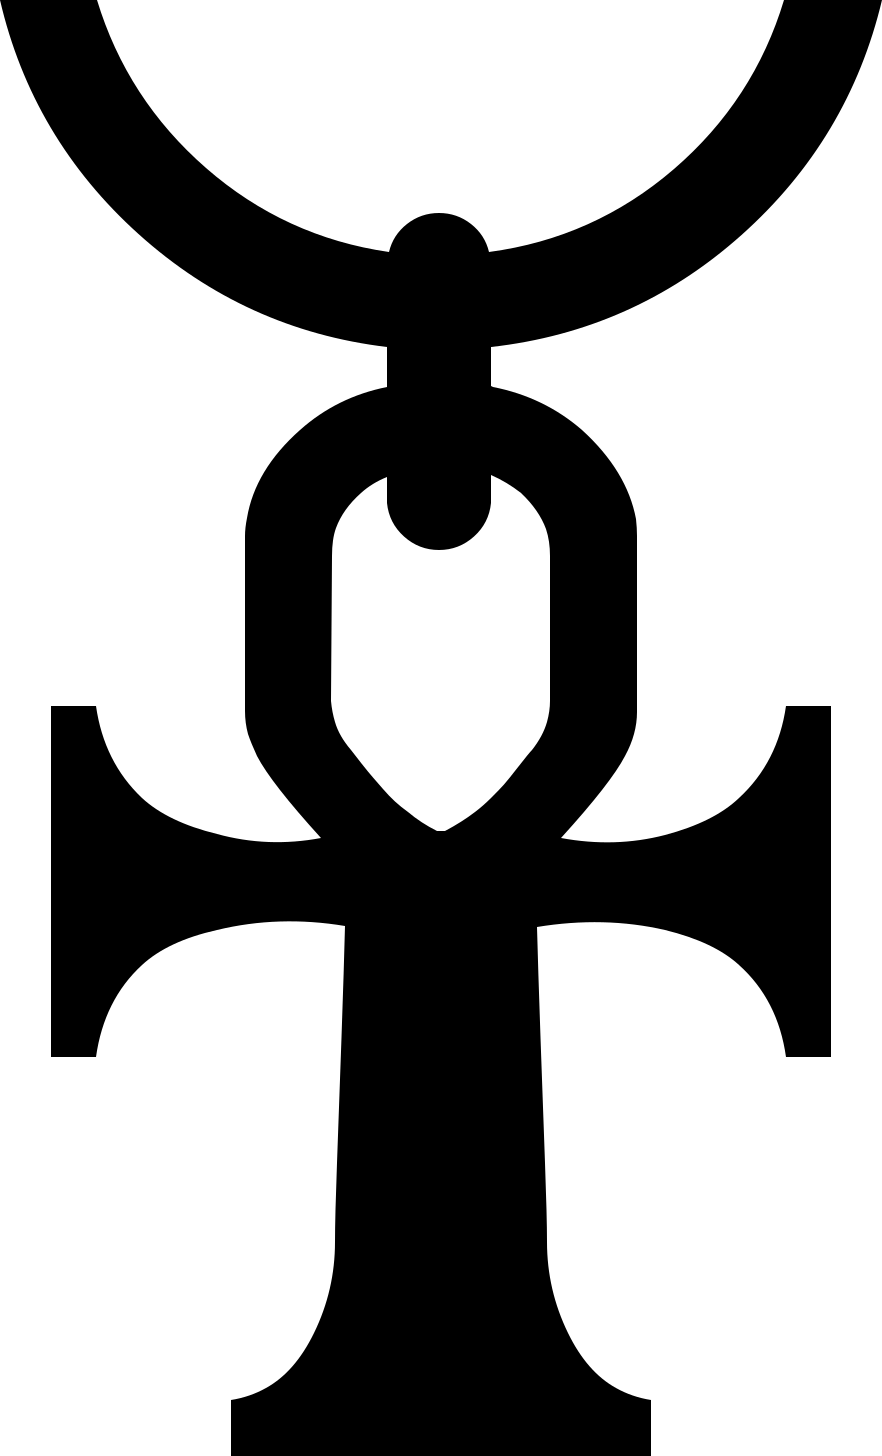
\includegraphics[width=1.2\linewidth]{\cards/artifact.png}};
    \draw (-1.3, 2.1) node {\encircle{1}};
    \draw (1.3, -0.9) node {\encircle{2}};
    \draw (1.4, 2.6) node {\encircle{3}};
    \draw (-1, -1.9) node {\encircle{4}};
  \end{tikzpicture}
  \end{scriptsize}
  \footnotesize
    \null\hfill\textbf{\textit{\textcolor{darkcandyapplered}{Major Artifact}}}
  \columnbreak
  \begin{center}
    \phantom{\ldots}\\
    \phantom{\ldots}
    \begin{scriptsize}
    \begin{tikzpicture}
      \draw (0, 0) node {\includegraphics[width=0.6\linewidth]{\cards/minor_artifact.png}};
      \draw (-0.7, 0.5) node {\encircle{3}};
    \end{tikzpicture}
    \end{scriptsize}\\
    \phantom{\ldots}\textbf{\textit{\textcolor{darkcandyapplered}{Minor Artifact}}}\\
    \vspace{3em}
    \phantom{\ldots}
    \begin{scriptsize}
    \begin{tikzpicture}
      \draw (0, 0) node {\includegraphics[width=0.6\linewidth]{\cards/relic_artifact.png}};
      \draw (-0.7, 0.5) node {\encircle{3}};
    \end{tikzpicture}
    \end{scriptsize}\\
    \phantom{\ldots}\textbf{\textit{\textcolor{darkcandyapplered}{Relic Artifact}}}
  \end{center}
\end{multicols*}
\begin{multicols}{2}
  \footnotesize
  \begin{itemize}
    \item[\textbf{1.}] Name
    \item[\textbf{2.}] Effect
    \columnbreak
    \item[\textbf{3.}] Level
    \item[\textbf{4.}] Fluff
  \end{itemize}
\end{multicols}

\begin{center}
  \vspace*{\fill}
  {\transparent{0.2}\includegraphics[width=0.9\linewidth]{\art/diplomats_ring.png}}
  \vspace*{\fill}
\end{center}

\pagebreak

\begin{expansion}{stronghold}
\subsection*{\pagetarget{Spell Scroll Cards}{Spell Scroll Cards}}

During setup shuffle 10 of the Spell Scroll Cards into the Artifact Deck.
Set the remaining 10 Cards aside to form a Spell Scroll Deck.
Some locations or Scenario effects may call for them later.
\vspace*{1em}

{
    \medskip
    \centering
    \includegraphics[width=0.7\linewidth]{\cards/test_spellscroll.png}\\
    \medskip
    \footnotesize
    \begin{center}
         \textbf{\textit{\textcolor{darkcandyapplered}{Spell Scroll Card}}}
    \end{center}
}

\vspace*{1em}
When you gain a Spell Scroll, place it next to your Hero Card, take the 2 top Cards from the Spell Deck and place them face-down on the Spell Scroll.
You can look at these Spells at any time and they don't count toward your Hand \svg{hand} Limit.
You can only have 2 Spell Scrolls at a time.
If you gain a third one, draw the new Spells normally and then decide whether to discard the newly gained Spell Scroll or replace one you already have (including all Spells on it).

\medskip

You can play Spells from a Spell Scroll like any other Spell with the following exceptions:
\begin{itemize}
    \item They don't count towards your Spell Limit.
    You can also play a Spell from your hand during this Combat Round.
    \item You can only use the Spell's lowest Power \svg{empower} effect.
    You can't Empower the Spell with \svg{empower} from any source.
    % What, if the lowest Power is 1? Can it be still played or not?
    \item They can't be used to increase the \svg{empower} of another Spell.
\end{itemize}
\end{expansion}
\columnbreak
\begin{expansion}{stronghold}
    \begin{itemize}
    \item You can sell Spell Scrolls at a Trading Post for 2 \svg{gold} per each Spell on it.
    %Is it a new option at a Trading Post or can i combine it with other actions in a single visit?
    \item After using or selling those Spells, the Spell Card is \textbf{removed}, not discarded.
\end{itemize}

If the last Spell on a Spell Scroll is used or sold, place the Spell Scroll back in its Deck.
\end{expansion}
\vspace*{1em}
\begin{expansion}{rampart,cove}
  \subsection*{\pagetarget{War Machines}{War Machines}}

  War Machines\index{War Machines} are permanent Cards that can be bought at either a \pagelink{Trading Post}{Trading Post} or a \pagelink{War Machine Factory}{War Machine Factory}.
  If you buy one at the Trading Post, \textbf{you cannot use} any of the other normal functions of that Field during that Visit.
  War machines are also more expensive at the Trading Post.

  {
    \bigskip
    \centering
    \begin{scriptsize}
      \begin{tikzpicture}
        \draw (0, 0) node[inner sep=0] {\includegraphics[width=0.8\linewidth]{\cards/war_machine.png}};
        \draw (0.8, 3.6) node {\encircle{\phantom{.}1\phantom{.}}};
        \draw (0, -2.8) node {\encircle{\phantom{.}2\phantom{.}}};
        \draw (-1.2, -1.7) node {\encircle{\phantom{.}3\phantom{.}}};
        \draw (0.9, -1.7) node {\encircle{\phantom{.}4\phantom{.}}};
      \end{tikzpicture}
    \end{scriptsize}

    \footnotesize
    \textbf{\textit{\textcolor{darkcandyapplered}{War Machine Card}}}
    \begin{itemize}[itemsep=0pt, parsep=5pt, topsep=0pt, partopsep=0pt]
      \item[\textbf{1.}] Name
      \item[\textbf{2.}] Effect
      \item[\textbf{3.}] Cost in a War Machine Factory
      \item[\textbf{4.}] Cost in a Trading Post
    \end{itemize}
  }
\end{expansion}

\vspace*{\fill}

\subsection*{Searching Example}

\textit{Bob, playing as Deemer the Warlock, has built a Mage Guild during the previous Game Round, enabling him to now use his Spell Book Token to purchase additional Spells.}

\includegraphics[width=\linewidth]{\examples/deemer_receiving_spellbook.png}\par
\textit{He spends the token and pays the cost of 5 \svg{gold} indicated on his Town Board, allowing him to \textbf{Search (2)} the Spell Deck.}\par
\includegraphics[width=\linewidth]{\examples/deemer_spell_cost.png}\par
\filbreak
\textit{He now has the choice of either gaining the top Card of the Spell Card Discard Pile, or drawing the top two Cards of the Spell Deck and gaining one of them.
He is not interested in gaining the Spell Curse, which is on top of the Discard Pile, and instead decides to draw two Cards – a Magic Arrow and a Fireball.}
\includegraphics[width=\linewidth]{\examples/fireball_over_magic_arrow.png}\par
\textit{He decides to keep the Fireball, placing it into his hand and discarding the Magic Arrow into the Spell Discard Pile.}

\vspace*{\fill}

\hfill{\transparent{0.2}\includegraphics[width=0.8\linewidth]{\art/fire_magic.png}}

\end{multicols*}


\addsection{Resources}{\images/estates.png}
\hypertarget{Resources}{There} are three types of resources in the game: Gold \includesvg[height=10px]{\svgs/gold.svg}, Building materials \includesvg[height=10px]{\svgs/BuildMat.svg}, and Valuables \includesvg[height=10px]{\svgs/valuablegreater.svg}.
Resources are spent during the game to expand your \hyperlink{Town}{Town}, to recruit \hyperlink{Units}{Units}, and to purchase \hyperlink{spells}{Spells}.
You can gain Resources from the \hyperlink{Mines}{Settlements and Mines} that you have \hyperlink{Categories}{Flagged}, but also by playing cards and rolling Resource Dice \includesvg[height=10px]{\svgs/resource_die.svg}.
Whenever a player's resource production is increased or decreased, move that Resource's cube on its production track the appropriate number of spaces.\par
\begin{figure}[h]
  \centering
  \minipage[b]{0.32\textwidth}
    \centering
    
\includegraphics[scale=0.2]{\images/gold.png}
    \caption{{\textit{\textbf{\textcolor{purple}{Gold}}}}}
  \endminipage
  \minipage[b]{0.32\textwidth}
    \centering
    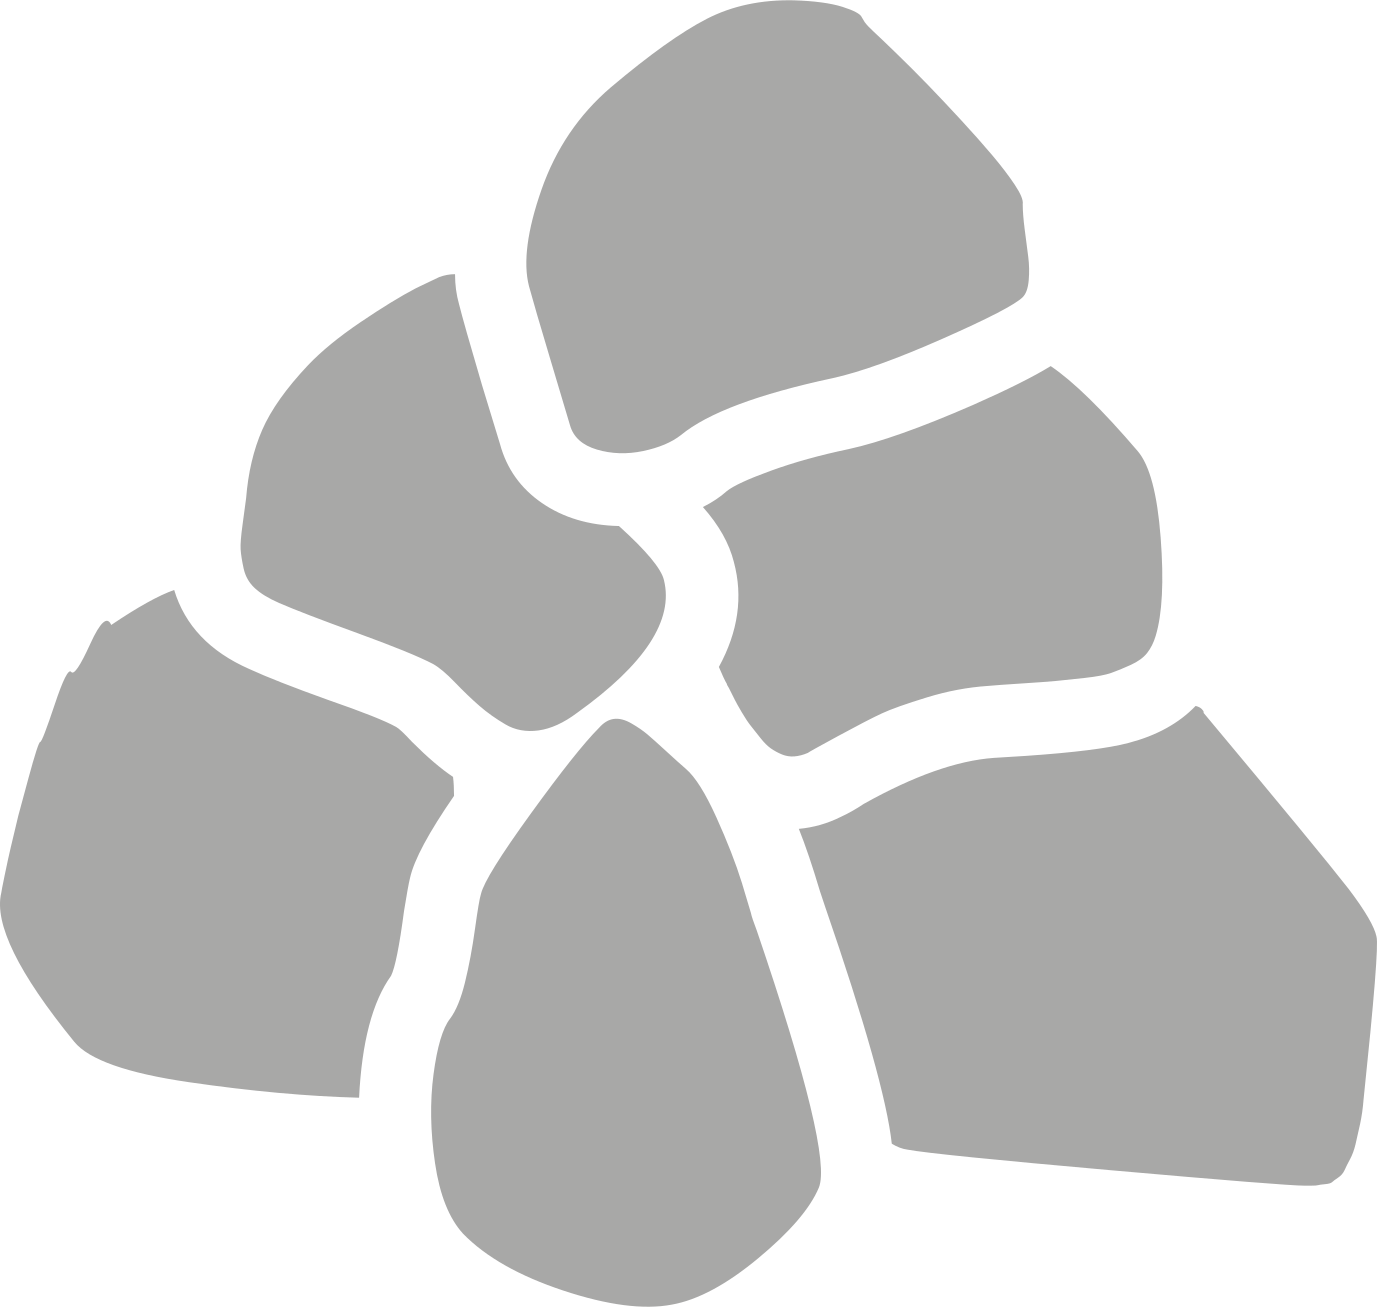
\includegraphics[scale=0.2]{\images/building_materials.png}
    \caption{{\textit{\textbf{{\textcolor{purple}{Building Materials}}}}}}
  \endminipage
  \minipage[b]{0.32\textwidth}
    \centering
    \includegraphics[scale=0.2]{\images/valuables.png}
    \caption{{\textit{\textbf{{\textcolor{purple}{Valuables}}}}}}
  \endminipage
\end{figure}
Players start each scenario with the number of resources indicated in that scenario’s set up.
Resources can also be \hyperlink{Trading}{traded}.
There's no limit to the amount of resources you can have.\bigbreak

\begin{minipage}[T]{0.38\textwidth}
    Possible Resource Die \includesvg[height=10px]{\svgs/resource_die.svg} results:\bigbreak
    \begin{itemize}
        \setlength\itemsep{10pt}
        \item \includesvg[height=15px]{\svgs/2BuildMat.svg} - 2 x Building Materials
        \item \includesvg[height=15px]{\svgs/4BuildMat.svg} - 4 x Building Materials
        \item \includesvg[height=15px]{\svgs/1valuables.svg} - 1 x Valuables
        \item \includesvg[height=15px]{\svgs/2valuables.svg} - 2 x Valuables
        \item \includesvg[height=15px]{\svgs/3gold.svg} 3 x Gold
        \item \includesvg[height=15px]{\svgs/6gold.svg} 6 x Gold
    \end{itemize}
\end{minipage}
\begin{minipage}[t]{0.48\textwidth}
    \shadowimage[width=0.88\textwidth]{\images/resource_board.png}
    \break
    \centering
    \footnotesize{\textbf{\textit{\textcolor{purple}{Resource production tracker}}}}
\end{minipage}\hfill


% !TeX spellcheck = en_US
\addsection{Town}{\skills/artillery.png}

\begin{multicols*}{2}

\hypertarget{Town}{Each} Faction has their own Town, which is located in the center of their Starting Tile.
The Town is your most important location, as many Scenarios \hyperlink{End}{may end} if it's \hyperlink{Categories}{Flagged} by an enemy Hero.\par
The contents of your Town and overall Faction status are represented by the Town Board.
It shows your currently built Buildings, Resource costs for future Buildings, your Resource incomes and status of Town Action Tokens.\par
All Factions are able to Build the following Buildings in their Town:
\begin{itemize}
  \item \textbf{City Hall} – Provides Resource income or a Faction-Specific Ability.
  \item \textbf{Citadel} – Allows you to Reinforce Units when using the Population Token.
Also \hyperlink{Walls}{protects your Town} when it is attacked.
  \item \textbf{Unit Dwellings} – Allows you to Recruit Units.
Dwellings have three Levels that unlock new Units, but which must be Built in the following order:\includesvg[height=10px]{\svgs/bronze.svg}\includesvg[height=10px]{\svgs/silver.svg}\includesvg[height=10px]{\svgs/Golden.svg}
  \item \textbf{Mage Guild} - gives you \hyperlink{spells}{Spells}.
  \item \textbf{Faction Building} - a Faction-Specific Building with a unique effect.
\end{itemize}
\textbf{A single Building} may be Built each Round by using the Build Token.
When you build a Building, pay its cost in Resources, flip the Build Token to its inactive side, and place the new Building’s Cardboard Piece into its proper slot on the Town Board.
If the Building has any immediate effects upon Building it, resolve them now.\par
Built Buildings are always represented by a symbol within a circle.
Buildings that can be built in the future are represented by a rectangle that contains the Building's cost in Resources.
Many Building Tiles are double-sided, and may later be upgraded and flipped to represent two different buildings at the same time. Such upgrades must be Built in order.\par
If a Town or Settlement is attacked by an enemy hero and your Hero is not also on that Field, you may immediately \textbf{pay 8 Gold} to fight a defending Combat \textbf{using only your Units}.
You cannot use your Deck during that Combat as your Main Hero is not present.
Paying this Gold represents the cost of transporting the army there.\par
When you \hyperlink{Categories}{Flag} a Town, take \hyperlink{End}{a Faction Cube} from its previous owner.

\vspace*{\fill}

\begin{center}
  \includegraphics[width=\linewidth]{\art/earthquake.png}
\end{center}

\vspace*{\fill}

\end{multicols*}


\addsection{Map Elements}{\images/logistics.png}

\begin{wrapfigure}{r}{0.5\textwidth}
  \includegraphics[width=0.9\linewidth]{\images/maptiles.png}
\end{wrapfigure}
Each Scenario is built using four types of Map Tiles.
Players always have a Faction-Specific Starting (I) Map Tile and may additionally have a number of face-down Far (II-III) Map Tiles which can be used to add new areas to the Scenario by spending MP.
Near (IV-V) and Center (VI-VII) Tiles are usually placed face down randomly during a Scenario’s set up and must be turned face up by spending MP when your Hero is next to them.
All face-down tiles should be selected randomly from the pool of possible Tiles and shuffled to keep their front side hidden.\par
The \textbf{roman numeral} of each tile describes the overall \textbf{difficulty of Neutral Units} on that tile, as well as the number of rewards players might expect to find on that Tile.
Starting (I) Tiles are the easiest while Center (VI-VII) Tiles are the most difficult.\par
\par

\begin{wrapfigure}{R}{0.5\textwidth}
  \begin{center}
  \includegraphics[width=0.47\textwidth]{\images/fields.png}
  \end{center}
\end{wrapfigure}
\subsection*{Map Tile Anatomy}
Each Map Tile is divided into 7 separate \textbf{Fields} that your Heroes can \textbf{Visit}.
When a Hero moves to a Field, they must immediately Visit it, or
first start a \hyperlink{Combat}{Combat} against the enemies guarding it before visiting.
Empty Fields do nothing when visited.
Solid yellow lines on a Field's edge cannot be passed through.
\hyperlink{Difficulty}{Roman numerals} written on a Field indicate that the Field is guarded by neutral enemies that must be fought to Visit it.\par

\clearpage

\subsection*{\hypertarget{Categories}{Location Categories}}
Visiting Fields provides Heroes with benefits such as gaining Resources or Cards.
There are three categories of Visitable Fields:
\begin{itemize}
  \item \textbf{Visitable} – Once you Visit this field, place a Black Cube on it.
    Treat it as an Empty Field as long as it has a Black Cube.
  \item \textbf{Flaggable} – These Fields can be directly captured by players and provide passive benefits.
    When you visit one, place a Faction Cube on it and gain a benefit.
    Enemy Heroes who Visit your Flagged Fields will replace your Cube with theirs to \textbf{steal} the Field’s effects.
    Allied Heroes treat Flagged Fields \textbf{as if they were empty}.
  \item \textbf{Revisitable} – You can Visit this Field multiple times.
    Do not place a Black Cube when you Visit it.
    You may pay 1 MP to Visit this Field again when your Hero occupies this Field.
\end{itemize}

See \hyperlink{All}{this section} for a list of all possible Fields and what they do.
\subsection*{\hypertarget{Placing}{Placing and Discovering New Tiles}}
When you Hero is adjacent to an undiscovered face down Tile, that Hero may spend 1 MP during your turn to flip and reveal that Tile.
You may then rotate the Tile as you see fit and place it back face-up.\par
In some Scenarios you will receive your own individual stack of Far (II-III) Map Tiles.
These can be placed on the map to expand the play area.
Tiles should be kept \textbf{hidden from all players} until they are about to be placed.
Placing a new Tile costs 1MP.
It must be placed adjacent to the Hero who spends the MP, and to at least two other existing Tiles.
New Tiles must also be positioned so that there is a valid path that eventually joins them with all other Tiles.
You may always rotate Map Tiles when placing them.\par
\begin{center}
  \includegraphics[width=\textwidth]{\images/placement.png}
\end{center}


% !TeX spellcheck = en_US
\addsection{Units}{\skills/leadership.png}

\begin{multicols*}{2}

\pagetarget{Units}{In}\index{Units} addition to their Hero and its associated deck, players also have \textbf{a deck of Unit Cards} which represent the armies moving with their Heroes.
Every Faction has access to \textbf{7 different Units}, each with unique stats and abilities.
Units are necessary for winning Combat and fulfilling Scenario goals.
Each Scenario's setup instructions indicate which Unit Cards should be included in your initial Unit Deck.
This Deck should be kept clearly separated from the rest of your Faction's Units.\par
Each Faction Unit is double-sided, with a weaker ``Few'' side, and a stronger ``Pack'' side.
``Few'' units may be upgraded to ``Packs'' by \textbf{Reinforcing} them, while taking damage can subsequently reduce a Unit back to its ``Few'' side.
Units should be always kept on their correct side when moved or inspected.\par
A player's Unit Deck may have any number of Units, but \textbf{only up to 5 Units} can be selected to fight during \pagelink{Combatsetup}{Combat Setup}.
If a Unit is defeated in Combat, \textbf{discard it} from your Unit Deck.\par
Units may be Recruited\index{Recruiting} and Reinforced\index{Reinforcing} by flipping the Population Token\index{Population Token} and paying the Unit's Recruitment \includesvg[height=10px]{\svgs/pay.svg} or Reinforcement \includesvg[height=10px]{\svgs/reinforce.svg} cost.
When you do so, you can instantly Recruit and Reinforce \textbf{any number} of times, provided you have enough Resources and the prerequisite Buildings to do so.\par
\textbf{Recruiting} a Unit requires that your Town has a Dwelling of that Unit's Level (\includesvg[height=10px]{\svgs/bronze.svg}\includesvg[height=10px]{\svgs/silver.svg}\includesvg[height=10px]{\svgs/golden.svg}).
\textbf{Reinforcing} requires that your Town has a Citadel in addition to a Dwelling of that Unit's Level.\par

\note{13}{
  Any effects which instruct you to Reinforce \textbf{do not} require spending your Population Token nor owning a Citadel or any Dwellings.\par

  \medskip

  If all Units in your Unit Deck are defeated, \textbf{immediately} replace your Unit Deck with the starting Units\index{Starting Units} of the Scenario. Defeated Faction Units can always be Recruited again with another use of the Population Token.
}

\vspace*{\fill}
  \iftoggle{printable}{}{\hspace{1em}}
\includegraphics[width=1.2\linewidth]{\art/gorgone.png}

\clearpage

\end{multicols*}
\begin{multicols}{2}
\subsection*{Unit Card Anatomy}

\vspace{0pt}

\includegraphics[height=30px]{\images/attack.png} \textbf{Attack} – The amount of damage this Unit deals when it attacks.\par
\includegraphics[height=30px]{\images/defense.png} \textbf{Defense} - The amount by which this Unit reduces oncoming Attack damage.
Does not apply to damage received from Spells or other non-attack effects.\par
\includegraphics[height=30px]{\images/hp.png} \textbf{\pagetarget{HP}{HP}} - The amount of damage required to defeat the Unit.
``Few'' Units are discarded from Combat and their owner's Unit Deck when defeated.
``Pack'' Units are turned back to ``Few'' Units, with any excess damage placed on their ``Few'' side.
Units retain their ``Few'' or ``Pack'' status between Combats.
All damage is healed from all Units at the end of Combat.\par
\includegraphics[height=30px]{\images/initiative.png}{\pagetarget{Initiative}{\textbf{Initiative}}} - Determines when the Unit Activates during Combat.
Units with a higher Initiative Activate first.

\vfill
\hspace{-2em}
\includegraphics[width=\linewidth]{\art/behemoth.png}

\begin{center}
  \includegraphics[width=\linewidth]{\cards/units.png}
\end{center}
\vspace{-1em}
\begin{multicols*}{2}
  \footnotesize
  \begin{center}
    \textbf{\textit{\textcolor{darkcandyapplered}{Unit Card (Few)}}}
  \end{center}
  \begin{itemize}
    \item[\textbf{1.}] {Name}
    \item[\textbf{2.}] {Tier}
    \item[\textbf{3.}] {Type}
    \item[\textbf{4.}] {Attack}
    \item[\textbf{5.}] {Defense}
    \item[\textbf{6.}] {HP}
  \end{itemize}
  \columnbreak
  \begin{center}
    \textbf{\textit{\textcolor{darkcandyapplered}{Unit Card (Pack)}}}
  \end{center}
  \begin{itemize}
    \item[\textbf{7.}] {Initiative}
    \item[\textbf{8.}] {Recruitment cost}
    \item[\textbf{9.}] {Reinforcement cost}
    \item[\textbf{10.}]{Pack symbol}
    \item[\textbf{11.}]{Special Ability}
    % \item[\textbf{\phantom{.}}] \phantom{.}
  \end{itemize}
\end{multicols*}

\bigbreak

Most Units have a \textbf{special ability}\index{Special Ability}:\par
\begin{itemize}[wide]
  \item\textbf{Activation} \includesvg[height=10px]{\svgs/activation.svg} resolves when the Unit is Activated.
  \item\textbf{Attack} \includesvg[height=10px]{\svgs/unit_attack.svg} resolves when the Unit attacks during its Activation.
    In case of multiple attacks, resolve the effect for \textbf{the first attack only}.
  \item\textbf{Other} \includesvg[height=10px]{\svgs/unit_other.svg} may be resolved instead of the Unit's normal Activation.
    It replaces all movement and/or attacking.
  \item\textbf{Passive} \includesvg[height=10px]{\svgs/unit_passive.svg} resolves whenever its condition is met.
  \item\textbf{Retaliate} \includesvg[height=10px]{\svgs/unit_retaliate.svg} resolves when the Unit retaliates.
  \item In any other cases without one of the above icons, the Unit's ability is used according to its text.
    Units may also use symbols representing \pagelink{Card Effects}{Card Effects}.
\end{itemize}

\vspace*{\fill}

\columnbreak

\subsection*{\pagetarget{Unittype}{Unit Types}}
There are three types of Units:
\begin{itemize}
  \item \textbf{Ground}\index{Ground Units} \includesvg[height=10px]{\svgs/unit_ground.svg} Units may move up to 3 spaces and then attack an adjacent enemy.
  \item \textbf{Flying}\index{Flying Units} \includesvg[height=10px]{\svgs/unit_flying.svg} Units may move up to 3 spaces, \textbf{ignoring Combat Obstacles}, and then attack an adjacent enemy.
  \item \textbf{Ranged}\index{Ranged Units} \includesvg[height=10px]{\svgs/unit_ranged.svg} Units may attack \textbf{any enemy Unit anywhere} and then move up to 1 space OR move up to 1 space without attacking.
\end{itemize}
If a \includesvg[height=10px]{\svgs/unit_ranged.svg} Unit is next to an enemy Unit, its attack target \textbf{must be} that adjacent enemy.
When attacking an adjacent enemy in this way, the \includesvg[height=10px]{\svgs/unit_ranged.svg} Unit suffers a Combat penalty\index{Combat Penalty}: throw two Attack Dice (instead of one) and \textbf{apply the smaller result}.\par
This penalty is also applied if the \includesvg[height=10px]{\svgs/unit_ranged.svg} Unit attacks from its own Backline into the enemy's Backline.
Walls and Gates may also \pagelink{Walls}{reduce} the damage from  \includesvg[height=10px]{\svgs/unit_ranged.svg} attacks.

\subsection*{\pagetarget{Neutral Units}{Neutral Units}}
Neutral Units\index{Neutral Units} guard the various locations on the Game Map.
Starting and winning Combat against them is necessary to Visit most Locations.
Neutral Units are spread into four different tiers, each with their own Deck.
In addition to \includesvg[height=10px]{\svgs/bronze.svg}, \includesvg[height=10px]{\svgs/silver.svg} and \includesvg[height=10px]{\svgs/golden.svg}, there are also Azure \includesvg[height=10px]{\svgs/azure.svg} Neutral Units which are the strongest in the game.\par
Each of these Decks should always be kept separate from each other and shuffled during setup.
If a Neutral Unit Deck ever runs out of Cards, reshuffle the discard into a new Deck.
When a Combat against Neutral Units starts, draw \pagelink{Difficulty}{the appropriate number} of Units from each tier to take part in that Combat.\par
It is possible for players to gain Neutral Units to their Unit Deck through various effects, such as Scenario-Specific Rules or the Diplomacy Ability Card.
\textbf{Neutral Units cannot be Reinforced}, as they are single sided.
Whenever a Neutral Unit is defeated from anywhere, place it into the appropriate Neutral Discard Pile.\par

\note{8}{
  Having a \includesvg[height=10px]{\svgs/golden.svg} Dwelling built in your Town allows you to draw an \includesvg[height=10px]{\svgs/azure.svg} Unit Card using the basic (top) effect of a Diplomacy Ability Card.
  This effect does not apply to Dungeon's Portal of Summoning.
}

\end{multicols}

\hommtable{13}{
  \begin{tabularx}{\linewidth}{XXXXX}
    & \darkcell{Town Building} & \darkcell{Castle} & \darkcell{Dungeon} & \darkcell{Necropolis} \\
    \darkcell[1.6]{\includesvg[height=12px]{\svgs/bronze.svg} \\ Bronze Units} &
      \lightcell[1.6]{Tier 1 \\ Dwelling} &
      \lightcell[1.6]{Halberdiers, Marksmen, Griffins} &
      \lightcell[1.6]{Troglodytes, Harpies, Evil Eyes} &
      \lightcell[1.6]{Skeletons, Zombies, Wraiths} \\
    \darkcell[1.2]{\includesvg[height=12px]{\svgs/silver.svg} \\ Silver Units} &
      \lightcell[1.2]{Tier 2 \\ Dwelling} &
      \lightcell[1.2]{Crusaders, Zealots} &
      \lightcell[1.2]{Medusas, Minotaurs} &
      \lightcell[1.2]{Vampires,\\ Liches} \\
    \darkcell[1.2]{\includesvg[height=12px]{\svgs/golden.svg} \\ Gold Units} &
      \lightcell[1.2]{Tier 3 \\ Dwelling} &
      \lightcell[1.2]{Champions, Archangels} &
      \lightcell[1.2]{Manticores, Black Dragons} &
      \lightcell[1.2]{Dread Knights, Ghost Dragons} \\
  \end{tabularx}
}

\clearpage


\begin{multicols}{2}

\includegraphics[width=\linewidth]{\art/lich.jpg}

\subsection*{Gameplay Example}

\textit{Bob, playing as Alamar the Warlock, casts a Magic Arrow against Alice's pack of Skeletons, Empowering \includesvg[height=10px]{\svgs/empower.svg} the Spell by 2 with the Expert  Effect \includesvg[height=10px]{\svgs/expert.svg} of a Power Card.}

\medskip

\includegraphics[width=\linewidth]{\examples/alamar_empowering_magic_arrow.png}

\medskip

\textit{The Skeletons take 3 damage \includesvg[height=10px]{\svgs/damage.svg} from the Spell.
  Their Defense \includesvg[height=10px]{\svgs/defense.svg} of 1 does not reduce the damage, because it only applies against attacks.
  The Skeletons have a HP \includesvg[height=10px]{\svgs/health_points.svg} of only 2, so they are now turned to their ``Few'' side and 1 leftover damage \includesvg[height=10px]{\svgs/damage.svg} is placed on them.
}

\bigskip

\includegraphics[width=\linewidth]{\examples/skeletons_flipped.png}

\end{multicols}


\addsection{Combat}{\images/sword.png}
\hypertarget{Combat}{Combat} starts whenever heroes encounter enemy heroes or units, and takes place on the separate combat board.
Combat with \textbf{neutral units} starts when a hero moves to an unvisited field with a roman numeral, which signifies the \hyperlink{Difficulty}{type and number} of Neutral units guarding that field.
Combat with \textbf{another player} can start in two ways:
\begin{itemize}
  \item You move into any Field containing one of their Heroes.
  \item You move into a Town or Settlement owned by them.
\end{itemize}
Players are able to start multiple combats during their turn.

\subsection*{\hypertarget{Combatsetup}{Combat setup}}

% TODO info about battlefield expansion
Combat takes place on the 4 x 5 combat board, which consists of two backlines and two frontlines on opposite ends and a middle row.
Follow these steps when fighting against \textbf{neutral units}:

\begin{itemize}
  \item Choose one of the combat board’s sides as your own.
Place up to 5 of your unit cards freely onto the back- and frontline of that side.
  \item Check the difficulty table and draw the corresponding number of neutral unit cards from their decks.
  \item The neutral units are placed differently depending on the game mode:
  \item In \textbf{clash} or \textbf{alliance} scenarios, the enemy player sitting to your right controls the Neutral Units and decides their placement.
Ranged units must be placed in the backline if possible.
  \item In \textbf{campaign} or \textbf{co-op} scenarios, units are placed from left to right from the player's perspective.
First, place any ranged units in the backline.
Then, place any flying or ground units in the frontline.
If there's not enough room to place a unit in its correct line, place them in the other one.
Units must be placed in decreasing initiative order.
If there's a tie, place higher tier units first.
If there's still a tie, the players decide the placement order.
\end{itemize}
Unit setup when fighting \textbf{other players}:
\begin{itemize}[wide]
  \item The attacking player places up to 5 units on their chosen side of the combat board, followed by the defender.
  \item If the combat takes place in a town with a citadel, the defender adds the \hyperlink{Walls}{wall, gate and arrow tower} cards after placing their units.
\end{itemize}

\clearpage
\subsection*{\hypertarget{Combatterminology}{Combat terminology}}
The following terms are used in this rule book and by the unit and other cards to describe effects
and elements during combat:\par
\textbf{Attacking playe}r – The player who started the combat by moving their hero.\par
\textbf{Defending player} – The player whom combat was started against.\par
\textbf{Activation} – A unit activates when it is next in the initiative order.\par
\textbf{Adjacent unit} – A unit is directly adjacent to another if it is one space away in a cardinal direction (nondiagonal).\par
\textbf{Combat round} – A full cycle of all units of each player being activated.\par
\textbf{Combat obstacles} – Every card placed on the combat board counts as a combat obstacle.
Obstacles block the movement of all non-flying units.\par
\textbf{Attack die} – A red die whose results range from -1 to +1.
Roll the die whenever a unit attacks and
add the result to the unit’s attack value.\par
\textbf{\hypertarget{Retaliate}{Retaliation attack}} – If a unit survives an attack by an adjacent unit, it performs an attack on that unit.
Each unit can perform only 1 retaliation attack per combat round.
Retaliation attacks function identically to normal attacks, but they cannot cause another retaliation attack.
Mark units which have performed a retaliation attack this round with a black cube.\par

\textbf{Paralysis} \includesvg[height=10px]{\svgs/paralysis.svg} – Effects which paralyze a unit place the paralysis token on them.
A paralyzed unit
skips its next activation and removes the token instead.
If it is attacked or takes any damage before that time, remove the paralysis token from that unit.\par
\textbf{\hypertarget{Defend}{Defend}} \includesvg[height=10px]{\svgs/defense.svg} – When a unit with a defense token is attacked, make another roll with the attack die
after the initial attack roll.
If you roll a “+1”, the defending unit gains an extra 1 defense for this attack.
If a unit has a defense token at the start of its activation, discard it.
That unit cannot take another defense action during that activation.

\subsection*{\hypertarget{CombatCards}{Using cards during combat}}
You may only use \textbf{one spell per combat round}.
Other card types can be used as many times as you want to.
Ongoing \includesvg[height=10px]{\svgs/ongoing.svg} and \includesvg[height=10px]{\svgs/activation.svg} activate effects can be used only when activating one of your units and before it attacks.
Ongoing effects last until end of combat or if the effect on the card is used up.
Instant \includesvg[height=10px]{\svgs/instant.svg} cards may be played at any time except between rolling the combat die and resolving damage unless otherwise stated.
Instant cards which increase a unit's statistics \textbf{last only for the duration of the currently activated unit's next attack}.
\subsection*{\hypertarget{Timelimit}{Combat time limits}}
Combat against neutral units has a time limit of \textbf{one Combat round}.
If the player cannot win the combat before the end of the current Combat round, they must either \hyperlink{Endcombat}{retreat} or spend 1 MP from the hero that started the combat in order to play another combat round.\par
\textbf{Note}: Combat against azure \includesvg[height=10px]{\svgs/azure.svg} units, other players or \hyperlink{AIrules}{AI heroes} have no time limit.
\clearpage
\subsection*{\hypertarget{Walls}{Defending a town with a citadel}}

When a town with a citadel is attacked, the defender adds the wall and gate obstacles in any order to the middle row of the combat board after placing their units.
The gate card is not an obstacle to the defending player.
The wall and gate cards can be destroyed by any adjacent \includesvg[height=10px]{\svgs/unit_ground.svg} or \includesvg[height=10px]{\svgs/unit_flying.svg} unit's attack.
Such attacks are always successful; do not roll the combat die when performing them.\par
Defending units standing on their own side and in the same column as a wall or a gate are partially protected from \includesvg[height=10px]{\svgs/unit_ranged.svg} attacks.
If they are targeted by a \includesvg[height=10px]{\svgs/unit_ranged.svg} attack performed from the opponent's side of the combat board, \textbf{reduce the attack's damage by 1}.
\par
The defender also gains the arrow tower unit card which is placed next to the combat board.
It can only be targeted by \includesvg[height=10px]{\svgs/unit_ranged.svg} attacks.
This unit is also destroyed if all wall and gate cards are destroyed.
The arrow tower cannot start a defensive combat by itself without other units and you do not need to destroy it in order to win when attacking.
\begin{figure}[h]
\centering
\includegraphics[width=0.25\linewidth]{\images/ranged_example.jpg}
\end{figure}\\
\begin{center}
\textit{A ranged attack from spaces 1-8 would be reduced by 1 when attacking the Halberdiers since that unit is standing on its own side behind a wall, and the attacker is on its own side.
If the attacker moved to spaces 9-11 or past them, the Halberdiers would no longer be protected.
The same is true if the Halberdiers moved one space to the right.}
\end{center}

\clearpage
\subsection*{Combat round structure}
Combat is divided into rounds, during which all of the units participating in that combat activate once in initiative order.
After each unit has activated once, a new combat round begins.
Combat lasts until all units on one side are eliminated, a player has to \textbf{retreat} when fighting neutral units, or a player \textbf{surrenders} to another player.
In \textbf{clash} and \textbf{alliance} scenarios, neutral units are always controlled by the next enemy player sitting to your right.
When controlling neutral units in this way they must always attack if possible, or if they can't, move as close to an enemy unit as possible.\par
Structure of a combat round:
\begin{itemize}
  \item Players activate their units in the decreasing order of unit \hyperlink{Initiative}{intiative}, starting with the next unit that has not yet been activated this combat round.
  \item When a unit activates, place a faction cube on it to indicate it has been activated this combat round.
  \item Activated units may move and attack according to their \hyperlink{Unittype}{type}.
  \item Instead of attacking, a unit may \hyperlink{Defend}{defend}.
  In Neutral Combat, the Neutral Enemy units cannot defend.
  \item Before a unit attacks, both players may \hyperlink{CombatCards}{play cards}. Cards are resolved in the order in which players decide to play them.
  \item After a unit's attack has been declared and all cards have been played that the players wish to play, roll the combat die.
    Modify the attacking unit's attack by the die's result, reduce it by the defending unit's defense, and then deal the rest as \hyperlink{HP}{damage} to the defending unit.
  \item If the defending unit was adjacent to the attacker, it \hyperlink{Retaliate}{retaliates} if it hasn't done so this round.
  \item Keep activating units until they've all been activated once.
After the last unit's activation, the combat round ends.
\end{itemize}
\subsection*{\hypertarget{Endcombat}{End of combat}}
When combat ends, all damage is healed from all surviving units.
Move any player owned units back to their unit deck and discard any leftover enemy neutral units.\par
In combat against \textbf{neutral units}, if the player defeats all opposing units they win the combat.
If the player \hyperlink{Timelimit}{runs out of time} or all of their units are defeated, they have to \textbf{retreat}.
When you retreat, move any surviving units back to your unit deck and move the hero that started the combat back to the field they last visited.
There are no other negative consequences.
Combat against \textbf{other players} can end in the following ways:
\begin{itemize}
  \item All units on one side are defeated.
    If a \textbf{main hero} is defeated in this way, the defeated player \textbf{loses morale} and has to \textbf{pay the winner} 5 gold.
    If a \textbf{secondary hero} is defeated instead, do not lose morale or pay any gold.
    In both cases, the defeated player also gives the winner one of their \hyperlink{End}{faction cubes}.
    Defeated main heroes are moved to a friendly town or settlement, while secondary heroes are removed from the game until recruited again.
  \item One player chooses to \textbf{surrender}.
You may surrender by paying the other player 10 gold when activating a unit.
Move your main hero or remove your secondary hero from the game as if you were defeated by losing your units.
There are no other direct consequences to surrendering; the winner does not gain a faction cube.
\textbf{Note}: You cannot surrender when defending a town.
\end{itemize}
When a secondary hero is attacked, they may also choose to be \textbf{instantly defeated} instead of fighting a combat in order to preserve their units.
When this happens, the attacker still receives a faction cube from the defeated hero.\par Defeating a main hero \hyperlink{End}{may eliminate} that player.

\subsection*{\hypertarget{Combatexperience}{Combat experience}}

Winning combat with your main hero usually grants them experience.
If either the difficulty of the neutral field or the level of a defeated enemy main hero was equal to your level, gain 1 \includesvg[height=10px]{\svgs/exp.svg}.
If they were higher than your level, gain 2 \includesvg[height=10px]{\svgs/exp.svg}.
Defeating a neutral combat which involved an azure \includesvg[height=10px]{\svgs/azure.svg} unit grants your Hero level 7 immediately.
If you gain multiple levels in this way, resolve their effects in order.\par
Secondary heroes cannot gain experience from winning a combat.
You also do not gain experience from defeating a secondary hero, or if an enemy hero surrenders to you.
\subsection*{\hypertarget{Quick}{Quick combat}}
If your hero’s level is higher than a field’s difficulty when combat against neutral units would begin, \textbf{no combat} takes place.
The player is considered to have beaten the neutral units by default and gains no rewards from the combat.

\subsection*{\hypertarget{AIrules}{Player vs AI}}
These rules apply when playing a \textbf{solo} game.
The AI combat rules for targeting and attacking are also used when playing a \textbf{cooperative} scenario.\par
Solo campaigns are played against AI Heroes who use two automated decks to play the game: the AI deck, and the spell deck.
The AI deck consists of cards that are similar in function to abilities and artifacts, but change depending on the game's \hyperlink{Difficulty}{difficulty}.
The spell deck should be used when instructed by the cards in the AI deck.
During combat against neutral enemies or AI heroes, their units follow an automatic set of instructions.
\textbf{Initiative rules} work identically.
When an \textbf{AI hero} activates a unit, drawn an AI card as its activation.\par
All AI controlled \includesvg[height=10px]{\svgs/unit_ground.svg} and \includesvg[height=10px]{\svgs/unit_flying.svg} units prioritize attacking units of the same tier.
If this is impossible, they attack the closest unit, prioritizing the lowest tier one.
\includesvg[height=10px]{\svgs/unit_ranged.svg} units prioritize attacking other \includesvg[height=10px]{\svgs/unit_ranged.svg} units of the same tier, then lower tier, and finally higher tier.
If there are no \includesvg[height=10px]{\svgs/unit_ranged.svg} for them to target they prioritize \includesvg[height=10px]{\svgs/unit_ground.svg} and \includesvg[height=10px]{\svgs/unit_flying.svg} units in the same tier order.
If there's more than one valid target, they attack the closest one.\par
If there's ever a tie between equally valid targets for any units, the players choose which unit is attacked.

\clearpage
\textbf{AI heroes} always start in their town's space unless otherwise stated.
They have 3MP and always use them to perform the following actions in decreasing priority:
\begin{itemize}
  \item Check if a player hero is on the same tile as the AI.
    If they are, spend all MP to move towards them in an attempt to begin combat.
  \item Check if there are any mines or settlements to flag on the map tile the AI hero is on.
    If there are any, move toward the closest one and flag it.
  \item Otherwise, move toward the player's town in an attempt to flag it.
Repeat this sequence until all MP is used.
\end{itemize}
\begin{wrapfigure}{R}{0.5\textwidth}
  \begin{center}
  \includegraphics[width=0.48\textwidth]{\images/ai_card.png}
  \end{center}
\end{wrapfigure}
AI heroes always automatically win combat against any neutral units, while simultaneously flagging or visiting all fields they happen to move through.
They gain no benefits from flagging or visiting fields.
AI heroes must discover face down map tiles as normal by spending 1 MP in order to move onto them.
The player chooses that tile’s orientation.\par
AI heroes cannot surrender and you cannot surrender to them.
They will always fight until they run out of units.
Winning combat against an AI hero does not grant any rewards unless stated by the scenario.
AI heroes do not have a town board, resources, or a hero card.
Their armies are static and defined by the scenario’s set up or other rules.\par
Any differences to the above will be described in any given scenario’s own rules.


% !TeX spellcheck = en_US
\addsection{AI rules}{\spells/fortune.png}

\begin{multicols}{2}

  AI rules apply to enemy heroes and all Combats, including against Neutral armies, in \textbf{Solo Campaigns} and \textbf{Cooperative} Scenarios.

  \pagetarget{AI Heroes}{\subheader{AI Heroes}}
  AI Heroes are used in the Campaigns.
  Their units are static and are defined by the Scenario: find the indicated unit cards when you start the scenario.
  If the unit indicates unit tier (\svg{bronze}, \svg{silver}, \svg{golden}, or \svg{azure}) instead of ``Few'' or ``Pack'', that's a Neutral Unit.

  During setup, if multiple AI Heroes use the same unit, and you do not have enough copies of its card, the AI Heroes must share it:
  set everything up without that card, and add it to the AI Hero's Army the moment you trigger Combat with them.

  AI Heroes cannot surrender and you cannot surrender to them;
  they will always fight until they run out of units.
  Winning Combat against an AI Hero does not grant any rewards unless stated by the Scenario.
  AI Heroes do not have a Town Board, Resources, or a Hero Board.

  \columnbreak
  \subsection*{AI Heroes Turns}
  Unless specified otherwise, AI heroes start in their Town, take turns after the player, and have 3 MP, always spending them to perform the following Actions in descending priority:
  \begin{itemize}
    \item If a player's Hero is on the same Tile as the AI, spend all MP to move towards them in an attempt to start Combat.
    \item If there are any Mines or Settlements the AI could flag on the same Tile, move towards the closest one.
    \item Otherwise, move toward the player's Town.
  Repeat this sequence until all MPs are used up.
  AI Heroes take their turn after the player.
  \end{itemize}

  AI Heroes always \textbf{automatically win Combat} against any Neutral Units, while simultaneously \textbf{flagging or Visiting all Fields} they happen to move through.
  They gain no benefits from any Fields.

  AI Heroes must discover face down Map Tiles as normal by spending 1 MP before moving onto them.
  The player chooses that Tile's orientation.
\end{multicols}

{\begin{center}
    \includegraphics[width=\linewidth,height=\textheight,keepaspectratio]{\art/harpy.jpg}
\end{center}}

\pagetarget{AI Deck}{\subheader{AI Decks}}
\begin{multicols*}{2}
  \begin{tikzpicture}
    \node (card) {\includegraphics[width=0.57\linewidth]{\cards/ai.png}};
    \begin{scope}[
      shift={(card.south west)},
      x={($(card.east) - (card.west)$)},
      y={($(card.north) - (card.south)$)},
      ]
      \draw (0.4, 0.85) node {\encircle{1}};
      \draw (0.8, 0.7) node {\encircle{2}};
      \draw (0.15, 0.5) node {\encircle{3}};
      \draw (0.55, 0.5) node {\encircle{4}};
      \draw (0.15, 0.3) node {\encircle{5}};
      \draw (0.55, 0.3) node {\encircle{6}};
      \draw (0.4, 0.1) node {\encircle{7}};
    \end{scope}
    \node [below=0pt of card.south] {\imagecaption{AI card}};
    \node [right=0pt of card.east] {
      \begin{minipage}[t]{0.47\linewidth}
        \scriptsize
        \begin{itemize}[itemsep=0.8em]
          \item[\textbf{1.}] Name
          \item[\textbf{2.}] Description
          \item[\textbf{3.}] Easy Modifier
          \item[\textbf{4.}] Normal Modifier
          \item[\textbf{5.}] Expert Modifier
          \item[\textbf{6.}] Impossible\\Modifier
          \item[\textbf{7.}] Card Type:\\
            \begin{itemize}[itemsep=0.5em]
              \item[\svg{might}] Might
              \item[\svg{magic}] Magic
              \item[\svg{skill}] Skill
            \end{itemize}
        \end{itemize}
      \end{minipage}
    };
  \end{tikzpicture}

  AI Heroes use two Decks during Combat: the \textbf{AI Deck}, and the \textbf{AI Spell Deck}.
  The AI Deck consists of three types of AI cards: Might \svg[12]{might}, Magic \svg{magic} and Skill \svg{skill}.
  Each Campaign Scenario lists the number and types of cards to include during setup.
  Choose these cards \textbf{randomly} when building the AI Deck.
  Shuffle the AI Deck before each Combat together with its discard pile.

  When an AI Hero \textbf{activates} a unit, draw an AI card\index{AI card} and follow its instructions before the unit \pagelink{AI Units}{moves and/or attacks}.
  If AI Deck is depleted during Combat, stop drawing from it.
  The effect of each AI card depends on the game's \pagelink{Difficulty}{Difficulty}.
  If an AI Hero is instructed to draw a card, they will draw and resolve \textbf{another card} from the AI Deck.

  If an AI card increased a unit's \svg{defense}, or triggered another card which increased it, the AI card stays attached to the unit until the first defense happens.
  % TODO: why attack isn't mention in expansion book? is it not the case for attack?
  % our old text here: The Might card \svg[12]{might} is attached to the unit until the first respective attack/defense happens.

  \subsection*{AI Deck sharing}
  If there are multiple AI Enemy Armies in the Scenario, but the rules don't specify which Enemy an AI Deck, an AI Spell Deck, or a Skill belongs to, you should assume it is shared between them.

  \subsection*{AI Magic cards and AI Spell Deck}
  Build the \textbf{AI Spell Deck} by separating the indicated Spells from the regular Spell Deck during setup.
  Shuffle the AI Spell Deck before each Combat together with its discard pile.

  Whenever an AI Magic \svg{magic} card is drawn, draw the next spell from the the AI Spell Deck, and cast it.
  Discarded spells go to its own AI Spell Discard pile.
  If the AI Spell deck empties before Combat ends, shuffle the AI Spell discard pile to form a new Spell deck.

  Sometimes in the AI Spell deck, there are more Spell cards than there are Magic cards in the AI Hero's deck.
  This is no mistake: not all spells need to be used, some are there for the sake of diversity.

  If the AI Hero is assigned a Spell card that is unavailable because it's your Hero's Deck, and you don't have another copy, substitute it with a \wikilink{spells/magic_arrow}{Magic Arrow} card.

  For certains spells it can be unclear how AI is supposed to use them.
  See \pagelink{AI Complex Spells}{Casting Complex Spells} for explanations.

  \subsection*{AI Skill cards}
  If Skill cards are included, search for and set aside the indicated card related to it (usually, an Ability).
  Whenever an AI Hero uses the AI Skill \svg{skill} card, use the skill card assigned to them in the Setup, but do not discard it afterwards.
  Contrary to the regular rules, the AI Hero can use the skill again, when instructed to do so by the AI deck.
  Discard the AI Skill \svg{skill} card as usual.

  AI Skill cards cannot be replaced, so if setup assigns the AI Hero a card that your Hero has and you don't have another copy,
  remove the needed card from your Hero's deck and \textbf{Search (3)} the respective card's deck to compensate your Hero for the loss.
\end{multicols*}

\pagetarget{AI Units}{\subheader{Combat against AI}}
\begin{multicols*}{2}
  These rules apply during Combat in \textbf{Solo}\index{Solo Mode} and \textbf{Cooperative} Scenarios.
  The rules for AI unit placement during setup are described in \pagelink{CombatAISetup}{Combat section}.

  When Neutral enemies or AI Heroes activate a unit, they follow a set of automatic instructions:\par

  \begin{itemize}
    \item If it's an AI Hero, draw and resolve the next \pagelink{AI Deck}{AI card}.

    \item Enemy Ground \svg{unit_ground} and Flying \svg{unit_flying} units prioritize attacking units of the \textbf{same} tier.
    If this is impossible, they attack the unit of a lower tier (in tier \textbf{descending} order, down to bronze), and if that is also impossible, they attack the unit of a higher tier (in tier \textbf{ascending} order).\par

    \textit{Example: \svg{golden}\svg{unit_ground} has this priority:
    \svg{golden}
    - \svg{silver}
    - \svg{bronze}
    - \svg{azure}.}

    \item Ranged \svg{unit_ranged} units prioritize attacking other Ranged \svg{unit_ranged} units of the same tier, then lower tier, and finally higher tier, using the same tier order as above.
    If there are no Ranged \svg{unit_ranged} units for them to target, they prioritize Ground \svg{unit_ground} and Flying \svg{unit_flying} units in the same tier order.\par

    \textit{Example: \svg{silver}\svg{unit_ranged} has this priority:
    \svg{silver}\svg{unit_ranged}
    - \svg{bronze}\svg{unit_ranged}
    - \svg{golden}\svg{unit_ranged}
    - \svg{azure}\svg{unit_ranged}
    - \svg{silver}\svg{unit_ground}\svg{unit_flying}
    - \svg{bronze}\svg{unit_ground}\svg{unit_flying}
    - \svg{golden}\svg{unit_ground}\svg{unit_flying}
    - \svg{azure}\svg{unit_ground}\svg{unit_flying}.}
  \end{itemize}

  In both cases, if there's more than one valid target, they attack the closest one.
  If there's ever a tie between equally valid targets, the player chooses which unit is attacked.\par

  Enemy units cannot \pagelink{Defend}{defend} unless instructed to.

  \columnbreak
  \subsection*{AI Siege}
  When the Walls and Gate are mentioned in Combat preparation but no additional information on how to arrange them is given, arrange them just like a human player would:
  place the Gate in front of the \svg{unit_ground} unit with the highest \svg{initiative}.
  By default, the units do not attack the Walls -- they would rather fly over them to attack their target or move towards it through the Gate.
  If it is not possible, they take a \pagelink{Defend}{Defend} Action.

  The \pagelink{Walls}{Arrow Tower} is treated like a Silver \svg{silver}\svg{unit_ranged} unit.
  However, if there are multiple equally valid targets, it will attack the target closest to perishing (has the smallest difference between \svg{health_points} and current \svg{damage}).

  \vspace*{\fill}

\end{multicols*}

\pagetarget{AI Complex Spells}{\subheader{Casting complex spells}}
\begin{multicols*}{2}
  In some campaigns enemies use a number of spells whose effects are not fully compatible with the standard use of AI Magic \svg{magic} cards.
  To fully use their effects, here are extended descriptions of how AI Heroes should use each of these spells.
  Of course, the scenario can override this.

  \subsection*{Spells attacking multiple targets}
  \textit{Examples: \wikilink{spells/fireball}{Fireball,} \wikilink{spells/chain_lightning}{Chain Lightning.}}

  When activated, target any unit with one or two adjacent units from the player’s army, prioritizing the groups where there are more higher-tier units.
  If there is more than one valid group, attack the one that is between the closest to perishing (has the smallest difference between \svg{health_points} and current \svg{damage}).
  If there is still more than one valid target, then you can choose which unit is attacked.
  If there are no player units adjacent to one another, target units that are not adjacent to any of the AI units.
  If that is also not possible, do not use this spell -- instead, skip the AI \svg{magic} card that activated this effect and put it on the bottom of the Enemy AI deck, then shuffle this spell back to the Enemy Spell deck.

  \subsection*{Instant Defense spells}
  \textit{Example: \wikilink{spells/stone_skin}{Stone Skin.}}

  When activated, put this card on the side of the Combat board, then put a Defense token on the unit with the highest \svg{defense} to represent the card’s effect -- it stays there until the defense is resolved.
  If there already is a Defense token on that unit, choose another one in the order of decreasing \svg{defense}.
  In case of a tie in \svg{defense} value, give preference to the unit of the highest tier and then to the greatest value of \svg{damage}.

  \columnbreak
  \subsection*{Healing spells}
  \textit{Example: \wikilink{spells/cure}{Cure.}}

  When activated, remove the \svg{damage} from the AI unit with the greatest value of \svg{damage} tokens, starting with the highest tier available.
  If no AI unit has any \svg{damage}, put the AI \svg{magic} card that triggered the spell at the bottom of the Enemy AI deck, then shuffle this Spell card back to the Enemy Spell Deck.

  \subsection*{Single-round buffs}
  \textit{Example: \wikilink{spells/fire_shield}{Fire Shield.}}

  % TODO FIFO or LIFO? do they all activate at the same time during first unit next round?
  When activated, check the tier of the unit on which you are about to cast the spell and count how many units of the same or higher tier there are on the board.
  If more than half of them have already activated this turn, do not cast the spell now -- instead, place it on the side of the Combat board and play it when the first AI unit activates in the next combat round.
  Skip drawing the AI card for that activation.

  \subsection*{Attack-weakening spells}
  \textit{Example: \wikilink{spells/weakness}{Weakness.}}

  When activated, if the AI’s activated unit is about to perform an attack that will provoke a Retaliation, cast this spell on the Retaliating enemy to lower their \svg{attack}.
  If the AI’s unit causes no Retaliation, do not cast this spell -- instead, ignore the AI card that activated the spell and put it at the bottom of the Enemy AI deck, then shuffle the Spell card back to the Enemy Spell deck.
\end{multicols*}


% !TeX spellcheck = en_US
\pagetarget{Difficulty}{\addsection{Difficulty}{\spells/fortune.png}}\index{Difficulty}

\begin{multicols}{2}

During setup, players must choose the game's Difficulty.
There are four different Difficulties, each with a different starting bonus\index{Starting Bonus} that players receive during step 16 of the setup:
\begin{itemize}
  \item \textbf{Easy} – Roll 2 \svg{resource_die} and receive Resources from both – OR – \textbf{Search} (2) the Artifact Deck, twice.
  \item \textbf{Normal} – Roll 2 \svg{resource_die} and receive the Resources from one of them – OR – \textbf{Search} (2) the Artifact Deck.
  \item \textbf{Hard} – Roll 1 \svg{resource_die} and receive the Resources on it – OR – reveal cards from the top of the Artifact Deck until you find 1 Minor Artifact and add it to your hand.
  \item \textbf{Impossible} – No starting bonus.
\end{itemize}
\columnbreak

Campaign missions have unique bonuses that \textbf{replace} the regular starting bonus.

All \textbf{Artifacts} received from a starting bonus should be placed into your \textbf{hand} and not shuffled into your Starting Deck.
If you searched for any Artifacts, shuffle the Artifact Deck and its Discard Pile\index{Discard Pile} together afterwards, and then discard one Artifact from the top to form the Artifact Discard Pile again.\par
The chosen difficulty also determines the number and type of neutral enemies that are encountered during Neutral Combat according to the \hyperlink{Difficulty Table}{table} at the back cover of the book.

\end{multicols}
\vspace*{\fill}
\includegraphics[width=\linewidth]{\art/enchanter.jpg}


% !TeX spellcheck = en_US
\pagetarget{Trading}{\addsection{Trading}{\art/ammo_cart.png}}\index{Trading}

\begin{multicols}{2}

\subsection*{Trading Post actions}
When visiting a \pagelink{Trading Post}{Trading Post Field} allows you to either:
\begin{itemize}
  \item trade multiple Resources with the game in accordance to the \hyperlink{Trade Table}{table at the back cover}, or
  \begin{expansion}[before skip balanced=0.4em,left=4mm]{rampart,cove}
    \item buy a \pagelink{War Machines}{War Machine}, or
  \end{expansion}
  \item \textbf{remove a single card} from your hand at the trading post to gain 1 \svg{gold}.
    \note{5}{Specialty, Statistic, Starting Ability and \wikilink{spells/magic_arrow}{Magic Arrows} \textbf{cannot be removed} in the Trading Post.}\par
\end{itemize}

In addition to the above, players can do following free actions an unlimited number of times during the same visit:
\begin{itemize}
  \item In \textbf{Cooperative Scenarios}: Resources may be given to other players.
  \begin{expansion}[before skip balanced=0.4em,left=4mm]{stronghold}
    \item Spells from a \pagelink{Spell Scroll Cards}{Spell Scroll card} can be \pagetarget{selling Spell Scrolls}{sold for 2~\svg{gold} each}.
      Remove sold Spells from the game.
  \end{expansion}
\end{itemize}
\columnbreak

\subsection*{Other Trading actions}
Certain game modes and game effects also allow you to trade:
\begin{itemize}
  \item In \textbf{Alliance Scenarios}, allies may trade Resources freely at any time on their Turns except during Combat.
  \item In \textbf{Alliance and Cooperative Scenarios}, allies may trade \textbf{Spell} and \textbf{Artifact} cards in any mix if they have Heroes on adjacent Fields.
    Only \textbf{cards from their hands} may be traded and you must give and receive an equal amount of cards.
  \item When other game effects allow you to \textbf{trade Resources} (e.g., \wikilink{events/marketplace}{Marketplace Event}), use the \hyperlink{Trade Table}{trade table} as well.
\end{itemize}
\medskip

\begin{center}
  {\transparent{0.2}\includegraphics[width=0.9\linewidth]{\art/black_market.png}}
\end{center}

\end{multicols}

\begin{center}
  \includegraphics[width=\linewidth]{\art/harpy.jpg}
\end{center}


\addsection{Scenario End}{\images/archery.png}
\hypertarget{End}{All} scenarios have their victory conditions listed in the scenario book.
In addition, it is always possible to be \textbf{eliminated} from any scenario in the following ways:
\begin{itemize}
  \item Play 3 full rounds without controlling a town or a settlement.
Count the number of rounds left using any suitable component.
  \item Lose combat with your main hero when you have no towns or settlements left, including when defending your last town or settlement.
\end{itemize}
Eliminated players are immediately out of the game.
Discard their faction cubes and heroes from the game map.
Treat the cards in their deck as being removed from the game for the rest of the scenario.
If you are eliminated, you may still participate in the game by controlling neutral units.
\textbf{Important}: If you eliminate all enemy factions you immediately win the scenario.\par
In \textbf{clash} scenarios, collecting \textbf{a faction cube} from every enemy player when there are 3 more players immediately wins you the game.
Other scenario specific rules may also modify the outcome of collecting faction cubes.


\addsection{Expansion Content}{\images/first_aid.png}

\begin{figure}[h]
  \begin{minipage}[t]{0.48\textwidth}
    \vspace{0pt}
    \subsection*{Schools of magic}
    Most expansions have cards which refer to schools of magic.
    All spell cards belong to one school: either air, fire, earth or water.
    There are multiple different cards and effects that interact with the schools in some way.
    The “magic arrow” spell can be considered to belong to every school but can only benefit from bonuses for a single school at a time.
    If relevant, you must select which school the magic arrow belongs to when casting it.
    Hero specialty cards are not spells even though some of them have a school of magic.
  \end{minipage}
  \begin{minipage}[t]{0.48\textwidth}
    \vspace{0pt}
    \centering
    \minipage[b]{0.5\textwidth}
      \centering
      \includegraphics[scale=0.17]{\images/school_of_fire.png}
      \caption{{\textit{\textbf{\textcolor{purple}{School of Fire}}}}}
    \endminipage
    \minipage[b]{0.5\textwidth}
      \centering
      \includegraphics[scale=0.17]{\images/school_of_water.png}
      \caption{{\textit{\textbf{\textcolor{purple}{School of Water}}}}}
    \endminipage
    \hfill\allowbreak%
    \bigbreak
    \minipage[b]{0.5\textwidth}
      \centering
      \includegraphics[scale=0.17]{\images/school_of_air.png}
      \caption{{\textit{\textbf{\textcolor{purple}{School of Air}}}}}
    \endminipage
    \minipage[b]{0.5\textwidth}
      \centering
      \includegraphics[scale=0.17]{\images/school_of_earth.png}
      \caption{{\textit{\textbf{\textcolor{purple}{School of Earth}}}}}
    \endminipage
  \end{minipage}
\end{figure}

\subsection*{Permanent cards}
Added by the stretch goals and Rampart expansions, explained \hyperlink{Playerdecks}{here}.

\begin{figure}[h]
  \begin{minipage}[t]{0.5\textwidth}
    \vspace{0pt}
    \subsection*{War machines}
    Added by the Rampart expansion.
    War machines are permanent cards that can be bought at either a trading post or a war machine factory.
    If you buy one at the trading post, you cannot use any of the other normal functions of that field during that visit.
    War machines are also more expensive at the trading post.
    \textit{I don't currently know if these have a player card back and are added to your hand like normal?}\par
    \smallskip
    \textbf{War Machine Factory}\\
    \shadowimage[width=0.8\textwidth]{\images/war_machine_factory.jpg}
      \caption{\scriptsize Category: \scriptsize\textbf{Revisitable}\\This location allows a Hero to buy a War Machine.}
  \end{minipage}
  \begin{minipage}[t]{0.4\textwidth}
    \vspace{0pt}
    \centering
    \begin{scriptsize}
      \begin{tikzpicture}
        \draw (0, 0) node[inner sep=0] {\makebox[\textwidth][c]{\shadowimage[width=0.8\textwidth]{\images/war_machine.jpg}}};
        \draw (1, 3.1) node {\encircle{\phantom{.}1\phantom{.}}};
        \draw (0, -2.9) node {\encircle{\phantom{.}2\phantom{.}}};
        \draw (-1.2, -1.8) node {\encircle{\phantom{.}3\phantom{.}}};
        \draw (1.1, -1.8) node {\encircle{\phantom{.}4\phantom{.}}};
      \end{tikzpicture}
    \end{scriptsize}
    \break
    \footnotesize{\textbf{\textit{\textcolor{purple}{War Machine Card}}}}
    \scriptsize
    \begin{multicols}{2}
      \begin{itemize}
        \item[\textbf{1.}] \textbf{Name}
        \item[\textbf{2.}] \textbf{Effect}
        \item[\textbf{\phantom{.}}] \phantom{.}
        \item[\textbf{3.}] \textbf{War Machine Factory cost}
        \item[\textbf{4.}] \textbf{Trading Post cost}
      \end{itemize}
    \end{multicols}
  \end{minipage}
\end{figure}

\begin{wrapfigure}{r}{0.5\textwidth}
  \begin{center}
  \includegraphics[width=0.48\textwidth]{\images/event.png}
  \end{center}
\end{wrapfigure}
\subsection*{Events}
Added by the Fortress expansion.
Event cards may be used in games with more than one player.
Shuffle the event deck during set up.
At the start of each resource round (except the first round), draw and read the next event card after receiving resources.
The first event is drawn by the starting player.
Change this player in a clockwise order every time a new event is drawn.
Resolve any effects in clockwise order starting with the player who drew the card.
Any cards which were revealed as a part of resolving an event should be shuffled back into their respective decks afterwards.

\begin{wrapfigure}{r}{0.5\textwidth}
  \begin{center}
  \includegraphics[width=0.48\textwidth]{\images/empowered_statistics.png}
  \end{center}
\end{wrapfigure}
\subsection*{Empowered statistic cards}
Added by the Inferno expansion.
These cards are more powerful versions of the normal statistics cards.
They have only one effect which is identical to the normal statistic's expert effect, but does not require using your \includesvg[height=10px]{\svgs/expert.svg}.

\subsection*{Summoning}
Some cards from the Inferno expansion may summon units during combat.
Place the summoned unit adjacent to the summoning unit.
Summoned units activate in the round they were summoned if their initiative is lower or equal to the initiative of the currently activated unit.
Otherwise, treat them as if they already activated this combat round.
After combat, unless stated otherwise, the summoned units are added to your unit deck.

\begin{wrapfigure}{r}{0.5\textwidth}
  \begin{center}
    \textbf{Random Town}
    \shadowimage[width=0.48\textwidth]{\images/random_town.jpg}
    \caption{\scriptsize Category: \scriptsize\textbf{Flaggable}}
  \end{center}
\end{wrapfigure}
\subsection*{Random town}
Added by the Inferno expansion.
When this field is revealed, all players roll 2 \includesvg[height=10px]{\svgs/resource_die.svg}.
The highest roller chooses an unused faction.
The random town is defended by units from that faction.
They have a pack of bronze, two packs of silver, and two "fews" of gold units.
Flagging it increases gold production by 10, which is also gained immediately if you are the first to flag it.


% !TeX spellcheck = en_US
\en{
  \addsection{All Map Locations}{\skills/earth_magic.png}
}
\pl{
  \addsection{Lokacje na mapie}{\skills/earth_magic.png}
}


\begin{multicols*}{2}

\en{\subsection*{Symbols on the Map}}
\pl{\subsection*{Ikony na mapie}}
\begingroup
  \renewcommand{\arraystretch}{1.5}
  \newcolumntype{Y}{>{\centering\arraybackslash}X}
  \begin{tabularx}{\linewidth}{Y m{0.7\linewidth}}
    \small
    \mbox{\textbf{I-VII}} &
      \en{Field Difficulty corresponding to the level of Neutral Units. }
      \pl{}
      \\
    \includesvg[height=15px]{\svgs/treasure.svg} &
      \en{Roll a Treasure Die and gain the indicated bonus.}
      \pl{}
      \\
    \includesvg[height=15px]{\svgs/resource_die.svg} &
      \en{Roll a Resource Die and gain the indicated Resources.}
      \pl{}
      \\
    \includesvg[height=15px]{\svgs/experience.svg} &
      \en{Gain one Experience Point.}
      \pl{}
      \\
    \includesvg[height=15px]{\svgs/spellpower.svg} &
      \en{Search (2) the Spell Deck.}
      \pl{}
      \\
    \includesvg[height=15px]{\svgs/artifact.svg} &
      \en{Search (2) the Artifact Deck.}
      \pl{}
      \\
    \includesvg[height=15px]{\svgs/morale_positive.svg} &
      \en{Gain Positive Morale.}
      \pl{}
      \\
    \includesvg[height=15px]{\svgs/morale_negative.svg} &
      \en{Gain Negative Morale.}
      \pl{}
      \\
    \includesvg[height=15px]{\svgs/movement.svg} &
      \en{Gain 1 Movement Point.}
      \pl{}
      \\
    {\huge\textbf{?}} &
      \en{Special effect, see \hyperlink{Revisitable Fields}{Revisitable} or \hyperlink{Other Fields}{Other} fields.}
      \pl{}
      \\
  \end{tabularx}
\endgroup

\bigskip

\begin{itemize}[itemsep=1em]
  \item [{\LARGE\textbf{+}}]
    \includesvg[height=0.8\baselineskip]{\svgs/gold.svg}/\includesvg[height=0.8\baselineskip]{\svgs/building_materials.svg}/\includesvg[height=0.8\baselineskip]{\svgs/valuablegreater.svg} —
    \en{Immediately gain the indicated Resource.}
    \pl{}
  \item [{\includesvg[height=15px]{\svgs/ongoing.svg}}]
    \includesvg[height=0.8\baselineskip]{\svgs/gold.svg}/\includesvg[height=0.8\baselineskip]{\svgs/building_materials.svg}/\includesvg[height=0.8\baselineskip]{\svgs/valuablegreater.svg} —
    \en{
      Increase the production of the indicated Resource.
      If it is \textbf{Flagged} for the first time, you also gain it immediately.
    }
    \pl{}
  \item [{\includesvg[height=0.8\baselineskip]{\svgs/pay_v2.svg}}]
    \includesvg[height=0.8\baselineskip]{\svgs/gold.svg}/\includesvg[height=0.8\baselineskip]{\svgs/building_materials.svg}/\includesvg[height=0.8\baselineskip]{\svgs/valuablegreater.svg} \includesvg[height=0.8\baselineskip]{\svgs/arrow_right.svg} —
    \en{The Player needs to pay the indicated Resource to gain something.}
    \pl{}
  \item [{\LARGE\textbf{2}}] {\LARGE\textbf{x}} —
    \en{Perform the {\LARGE\textbf{x}} action twice.}
    \pl{}
  \item [{\LARGE\textbf{2}}] \includesvg[height=0.8\baselineskip]{\svgs/treasure.svg}/{\LARGE\textbf{2}} \includesvg[height=0.8\baselineskip]{\svgs/resource_die.svg} \includesvg[height=0.8\baselineskip]{\svgs/arrow_right.svg}{\LARGE\textbf{1}} —
    \en{Roll 2 Treasure or Resource Dice and choose one to be resolved.}
    \pl{}
\end{itemize}

\phantom{\includesvg[height=1px]{\svgs/experience.svg}\includesvg[height=1px]{\svgs/spellpower.svg}}
\vspace*{\fill}
\columnbreak

\en{The effects of the following \textbf{Visitable} \hypertarget{All Map Locations}{fields} are explained by the symbols on the left:}
\pl{}

\medskip

{\centering
  \en{\phantom{j}\textbf{Artifact}\\}
  \pl{}
  \framedimage[\linewidth]{\map_locations/artifact_symbol.jpg}

  \bigskip

  \en{\phantom{j}\textbf{Resource}\\}
  \pl{}
  \framedimage[\linewidth]{\map_locations/resource_symbol.jpg}\\

  \bigskip

  \en{\phantom{j}\textbf{Treasure}\\}
  \pl{}
  \framedimage[\linewidth]{\map_locations/treasure_symbol.jpg}\\

  \bigskip

  \en{\phantom{j}\textbf{Fountain of Youth}\\}
  \pl{}
  \framedimage[\linewidth]{\map_locations/fountain_of_youth.jpg}\\

  \filbreak

  \en{\phantom{j}\textbf{Windmill}\\}
  \pl{}
  \framedimage[\linewidth]{\map_locations/windmill.jpg}\\

  \bigskip

  \en{\phantom{j}\textbf{Warrior's Tomb}\\}
  \pl{}
  \framedimage[\linewidth]{\map_locations/warriors_tomb.jpg}\\

  \bigskip

  \en{\textbf{Mystical Garden}\\}
  \pl{}
  \framedimage[\linewidth]{\map_locations/mystical_garden.jpg}\\

  \bigskip

  \en{\phantom{j}\textbf{Learning Stone}\\}
  \pl{}
  \framedimage[\linewidth]{\map_locations/learning_stone.jpg}\\

  \bigskip

  \en{\phantom{j}\textbf{Shrine of Magic Gesture/Incantation}\\}
  \pl{}
  \framedimage[\linewidth]{\map_locations/shrine_of_magic_whatever.jpg}\\

  \vspace*{\fill}
  \filbreak

  \en{\phantom{j}\textbf{Water Wheel}\\}
  \pl{}
  \framedimage[\linewidth]{\map_locations/water_wheel.jpg}\\

  \bigskip

  \en{\phantom{j}\textbf{Temple}\\}
  \pl{}
  \framedimage[\linewidth]{\map_locations/temple.jpg}\\

  \bigskip

  \en{\phantom{j}\textbf{Pandora's Box}\\}
  \pl{}
  \framedimage[\linewidth]{\map_locations/pandoras_box.jpg}\\
}

\vspace*{\fill}

\vspace{7.4em}

\note{10}{
  \en{
    The effects of Fields that allow you to \textbf{Search} for Spells or Artifacts, or where you must spend resources to use the Field's effect, are \textbf{always optional}.
    You must always place a Black Cube on such Visitable Fields even if you choose not to use that Field's effect.
  }
  \pl{}
}

\vspace*{\fill}

\pagebreak

\en{
  \subsection*{Towns, Mines and Settlements}
  \textbf{Towns} are always located in the center of a Starting (I) Tile.
  Flagging an enemy Town prevents their Secondary Heroes from spawning there and Main Heroes from moving there if defeated.
  Flagging a Town can cause \hyperlink{End}{Player Elimination}, and Scenarios typically have special rewards for Flagging them.
  Flagging a Town also gives you a \textbf{Faction Cube} from its original owner.
  Otherwise, Flagging a Town does not affect its original owner in any way.
  They do not lose access to their Town board or its functions.
  You also do not gain access to their Town board or Faction Units, unlike in the video game.
}
\pl{}

\begin{center}
  \framedimage[\linewidth]{\images/core_towns.jpg}
  \en{\textit{Towns from the core game.}}
  \pl{}
\end{center}

\medskip

\en{
  \hypertarget{Mines}{\textbf{Mines}}\index{Mines} are Flaggable Fields which increase a specific resource's income when Flagged.
  If you are the first one to Flag a mine, it also immediately provides you with its income.
  All mines have the \includesvg[height=10px]{\svgs/ongoing.svg} symbol and a picture of the Resource they produce next to it.
}
\pl{}

\begin{center}
  \includegraphics[width=0.55\linewidth]{\images/mine_example.png}\\
  \en{
    \textit{A mine that produces \includesvg[height=10px]{\svgs/valuablegreater.svg}, guarded by Level 3 Neutral Units.
      The first player to Flag this Field would immediately gain one \includesvg[height=10px]{\svgs/valuablegreater.svg} in addition to increasing their \includesvg[height=10px]{\svgs/valuablegreater.svg} income.
    }
  }
  \pl{}
\end{center}
\columnbreak

\en{
  \textbf{Settlements}\index{Settlement} act as a spawn point for Secondary Heroes, and as a place for Main Heroes to move to when defeated.
  When you Flag a Settlement, choose whether to increase your \includesvg[height=10px]{\svgs/gold.svg}, \includesvg[height=10px]{\svgs/building_materials.svg} or \includesvg[height=10px]{\svgs/valuablegreater.svg} income by one space.
  As with Mines, if you are the first player to Flag a Settlement, you \textbf{immediately} gain Resources equal to that increase in production.
  Mark the Settlement with an appropriate Resource Token to show which Resource it produces.
  When you Flag an enemy Settlement, you may change this Resource.\par
  Additionally, \textbf{instead of increasing Resource Production}, you may choose to \textbf{Reinforce} one of your \includesvg[height=10px]{\svgs/bronze.svg} or \includesvg[height=10px]{\svgs/silver.svg} Units immediately for half the normal cost, rounded up.
  If you were the first player to Flag the Settlement, Reinforce that Unit \textbf{for free} instead.
  Do not place any Resource Tokens on the Settlement if you choose to Reinforce.
}
\pl{}

\bigbreak

\begin{minipage}[h]{\linewidth}
  \centering
  \includegraphics[width=0.44\linewidth]{\map_locations/castle_settlement.png}
  \includegraphics[width=0.44\linewidth]{\map_locations/dungeon_settlement.png}
  \includegraphics[width=0.44\linewidth]{\map_locations/necropolis_settlement.png}
  \includegraphics[width=0.44\linewidth]{\map_locations/rampart_settlement.png}
  \includegraphics[width=0.44\linewidth]{\map_locations/fortress_settlement.png}
  \includegraphics[width=0.44\linewidth]{\map_locations/inferno_settlement.png}
  \includegraphics[width=0.44\linewidth]{\map_locations/tower_settlement.png}
  \par
  \en{
    \textit{All possible Settlements.
    Each is styled after a different Faction.
    They all work identically.}
  }
  \pl{}
\end{minipage}
\end{multicols*}
\bigbreak

\en{\subsection*{\hypertarget{Revisitable Fields}{Revisitable Fields}}}
\pl{}

\begin{figure}[H]
  \begin{minipage}[t]{0.47\textwidth}
    \vspace{0pt}
    \centering
    \en{\textbf{Library}\par}
    \pl{}
    \framedimage[\textwidth]{\map_locations/library.jpg}
    \caption{
      \en{
        \small Category: \textbf{Revisitable}\\You may
        \includesvg[height=8px]{\svgs/pay_v2.svg}
        3 \includesvg[height=8px]{\svgs/gold.svg}
        to Remove 1 Statistic Card from your hand or Discard Pile and replace it with any other Statistic Card.
        You may do this twice per Visit.
      }
      \pl{}
    }
  \end{minipage}\hfill
  \begin{minipage}[t]{0.47\textwidth}
    \vspace{0pt}
    \centering
    \captionsetup{singlelinecheck=off}
    \en{\phantom{j}\textbf{Black Market}\par}
    \pl{}
    \framedimage[\textwidth]{\map_locations/black_market.jpg}
    \caption[black market]{
      \en{
        \small Category: \textbf{Revisitable}\\Look at the top 4 cards from the Artifact Discard Pile.
        You may buy one of them for:
        \begin{itemize}
        \setlength\itemsep{-4pt}
          \item [5] \includesvg[height=8px]{\svgs/gold.svg} if it is a \textbf{Minor} Artifact
          \item [7] \includesvg[height=8px]{\svgs/gold.svg} if it is a \textbf{Major} Artifact
          \item [10] \includesvg[height=8px]{\svgs/gold.svg} if it is a \textbf{Relic} Artifact
        \end{itemize}
      }
      \pl{}
    }
  \end{minipage}
\end{figure}

\begin{figure}[H]
  \begin{minipage}[t]{0.47\textwidth}
    \vspace{0pt}
    \centering
    \en{\textbf{Sanctuary}\par}
    \pl{}
    \framedimage[\textwidth]{\map_locations/sanctuary.jpg}
    \caption{
      \en{
        \small Category: \textbf{Revisitable}\\
        Heroes on this Field cannot be attacked by other Heroes.
        Friendly Heroes can move through enemy Heroes on this Field but cannot stop here.
      }
      \pl{}
    }
  \end{minipage}\hfill
  \begin{minipage}[t]{0.47\textwidth}
    \vspace{0pt}
    \centering
    \en{\phantom{j}\textbf{Tavern}\par}
    \pl{}
    \framedimage[\textwidth]{\map_locations/tavern.jpg}
    \caption{
      \en{
        \small Category: \textbf{Revisitable}\\
        You can \includesvg[height=8px]{\svgs/pay_v2.svg}
        7 \includesvg[height=8px]{\svgs/gold.svg}
        to gain a Secondary Hero.
        Place their model on this Field.
        Then, choose one enemy player to discard 1 random card from their hand.
      }
      \pl{}
    }
  \end{minipage}
\end{figure}

\begin{figure}[H]
  \begin{minipage}[t]{0.47\textwidth}
    \vspace{0pt}
    \centering
    \en{\hypertarget{Trading Post}{\textbf{Trading Post}}\par}
    \pl{}
    \framedimage[\textwidth]{\map_locations/trading_post.jpg}
    \caption{
      \en{
        \small Category: \textbf{Revisitable}\\
        \textbf{Choose one}: \protect\hyperlink{Trading}{Trade} resources and Remove cards OR buy a \protect\hyperlink{War Machines}{War Machine}.
      }
      \pl{}
    }
  \end{minipage}\hfill
  \begin{minipage}[t]{0.47\textwidth}
    \vspace{0pt}
    \centering
    \en{\phantom{j}\hypertarget{War Machine Factory}{\textbf{War Machine Factory}}\par}
    \pl{}
    \framedimage[\textwidth]{\map_locations/war_machine_factory.jpg}
    \caption{
      \en{\small Category: \textbf{Revisitable}\\Buy a \protect\hyperlink{War Machines}{War Machine}.\phantom{.......}}
      \pl{}
    }
  \end{minipage}
\end{figure}

\begin{figure}[H]
  \begin{minipage}[t]{0.47\textwidth}
    \vspace{0pt}
    \centering
    \en{\phantom{j}\textbf{Stables}\par}
    \pl{}
    \framedimage[\textwidth]{\map_locations/stables.jpg}
    \caption{
      \en{
        \small Category: \textbf{Revisitable}\\
        Gain 1 MP \includesvg[height=8px]{\svgs/movement.svg}.
        It lasts for only one Turn.
        See \protect\hyperlink{Movement}{Movement Actions}.
      }
      \pl{}
    }
  \end{minipage}\hfill
\end{figure}

\begin{tikzpicture}[overlay]
  \node at (16, 4.5) {\includegraphics[width=0.5\linewidth]{\art/pegasi.png}};
\end{tikzpicture}

\en{\subsection*{\hypertarget{Other Fields}{Other Fields}}}
\pl{}

\begin{figure}[H]
  \begin{minipage}[t]{0.47\textwidth}
    \vspace{0pt}
    \centering
    \en{\textbf{Tree of Knowledge}\par}
    \pl{}
    \framedimage[\linewidth]{\map_locations/tree_of_knowledge.jpg}
    \caption{
      \en{
        \small Category: \textbf{Visitable}\\You may
        \includesvg[height=8px]{\svgs/pay_v2.svg}
         3 \includesvg[height=8px]{\svgs/valuablegreater.svg} or
         10 \includesvg[height=8px]{\svgs/gold.svg} to gain
         2 \includesvg[height=8px]{\svgs/experience.svg}.
      }
      \pl{}
    }
  \end{minipage}\hfill
  \begin{minipage}[t]{0.47\textwidth}
    \vspace{0pt}
    \centering
    \en{\textbf{Redwood Observatory}\par}
    \pl{}
    \framedimage[\linewidth]{\map_locations/redwood_observatory.jpg}
    \caption{
      \en{\small Category: \textbf{Visitable}\\Discover a face down Tile adjacent to this one.}
      \pl{}
    }
  \end{minipage}
\end{figure}

\begin{figure}[H]
  \begin{minipage}[t]{0.47\textwidth}
    \vspace{0pt}
    \centering
    \en{\phantom{j}\textbf{Grail}\par}
    \pl{}
    \framedimage[\linewidth]{\map_locations/grail.jpg}
    \caption{
      \en{
        \small Category: \textbf{Visitable}\\Gain a Grail Token.
        Only one Grail Token can exist in the game, do not gain another if this Field's Black Cube is removed or if there are multiple Grail Fields.
        The Token's effects are described in the Scenario's description.
        \phantom{\ldots\ldots\ldots}
      }
      \pl{}
    }
  \end{minipage}\hfill
  \begin{minipage}[t]{0.47\textwidth}
    \vspace{0pt}
    \centering
    \en{\phantom{j}\textbf{Market of Time}\par}
    \pl{}
    \framedimage[\linewidth]{\map_locations/market_of_time.jpg}
    \caption{
      \en{
        \small Category: \textbf{Visitable}\\ Remove one card from your hand.
        Then \textbf{Search (2)} the Ability, Spell, or Artifact Deck.
      }
      \pl{}
    }
  \end{minipage}
\end{figure}

\begin{figure}[H]
  \begin{minipage}[t]{0.47\textwidth}
    \vspace{0pt}
    \centering
    \en{\phantom{j}\textbf{Hill Fort}\par}
    \pl{}
    \framedimage[\linewidth]{\map_locations/hill_fort.jpg}
    \caption{
      \en{
        \small Category: \textbf{Visitable}\\
        You may immediately Reinforce one of your \includesvg[height=8px]{\svgs/bronze.svg} or \includesvg[height=8px]{\svgs/silver.svg} Units.
        The Reinforcement cost is reduced by 3 \includesvg[height=8px]{\svgs/gold.svg} to a minimum of 0.
      }
      \pl{}
    }
  \end{minipage}\hfill
  \begin{minipage}[t]{0.47\textwidth}
    \vspace{0pt}
    \centering
    \en{\phantom{j}\textbf{Prison}\par}
    \pl{}
    \framedimage[\linewidth]{\map_locations/prison.jpg}
    \caption{
      \en{
        \small Category: \textbf{Visitable}\\
        Gain a Secondary Hero.
        Place their model on this Field.
        If you already have a Secondary Hero, gain 3 \includesvg[height=8px]{\svgs/gold.svg} instead.
      }
      \pl{}
    }
  \end{minipage}
\end{figure}

\begin{figure}[H]
  \begin{minipage}[t]{0.47\textwidth}
    \vspace{0pt}
    \centering
    \en{\textbf{Magic Spring}\par}
    \pl{}
    \framedimage[\linewidth]{\map_locations/magic_spring.jpg}
    \caption{
      \en{
        \small Category: \textbf{Visitable}\\
        You may look at the top 3 Cards of your Discard Pile and return one of them to your Hand.
        Return the remaining cards to the top of your Discard Pile in any order.
      }
      \pl{}
    }
  \end{minipage}\hfill
  \begin{minipage}[t]{0.47\textwidth}
    \vspace{0pt}
    \centering
    \en{\phantom{j}\textbf{Witch Hut}\par}
    \pl{}
    \framedimage[\linewidth]{\map_locations/witch_hut.jpg}
    \caption{
      \en{
        \small Category: \textbf{Visitable}\\
        \textbf{Choose one}: Remove an Ability card from your hand OR look at the top card of the Ability Deck and put that card into your hand or into the Ability Deck Discard Pile.
      }
      \pl{}
    }
  \end{minipage}
\end{figure}

\begin{figure}[H]
  \begin{minipage}[t]{0.47\textwidth}
    \vspace{0pt}
    \centering
    \en{\phantom{j}\textbf{Obelisk}\par}
    \pl{}
    \framedimage[\linewidth]{\map_locations/obelisk.jpg}
    \caption{
      \en{
        \small Category: \textbf{Flaggable}\\
        The Obelisk's effects depend on the Scenario.
        When you Flag this Field, do not remove any enemy Faction Cubes; multiple players may have a Faction Cube on this Field.
      }
      \pl{}
    }
  \end{minipage}\hfill
    \begin{minipage}[t]{0.47\textwidth}
    \vspace{0pt}
    \captionsetup{singlelinecheck=off}
    \centering
    \en{\phantom{j}\textbf{Scholar}\par}
    \pl{}
    \framedimage[\linewidth]{\map_locations/scholar.jpg}
    \caption[scholar they]{
      \en{
        \small Category: \textbf{Visitable}\\
        Roll 1 Attack Die.
        Depending on the result, do the following:
        \begin{itemize}
          \setlength\itemsep{-0.2em}
          \item[ \textbf{+1}] - Gain a Statistic Card of your choice or Remove a Statistic Card from your hand.
          \item[\textbf{0}] - Draw 2 Cards from the Ability Deck, gain one of them and discard the other.
          \item[\textbf{-1}] - Draw 2 Cards from the Spell Deck, gain one of them and discard the other.
          \end{itemize}
       }
       \pl{}
     }
  \end{minipage}
\end{figure}

\begin{figure}[H]
  \begin{minipage}[t]{0.47\textwidth}
    \vspace{0pt}
    \centering
    \en{\textbf{Dragon Utopia}\par}
    \pl{}
    \framedimage[\linewidth]{\map_locations/dragon_utopia.jpg}
    \caption{
      \en{\small Category: \textbf{Flaggable}\\Effects depend on the Scenario.}
      \pl{}
    }
  \end{minipage}\hfill
  \begin{minipage}[t]{0.47\textwidth}
    \vspace{0pt}
    \centering
    \en{\textbf{University}\par}
    \pl{}
    \framedimage[\linewidth]{\map_locations/university.jpg}
    \caption{
      \en{
        \small Category: \textbf{Visitable}\\
        \includesvg[height=8px]{\svgs/pay_v2.svg} 6 \includesvg[height=8px]{\svgs/gold.svg} to \textbf{Search (4)} the Ability Discard Pile.
      }
      \pl{}
    }
  \end{minipage}
\end{figure}

\begin{multicols*}{2}

{\centering\phantom{Star Axis}\par}
\includegraphics[width=\linewidth]{\art/unicorn.jpg}

\columnbreak

\en{{\centering\textbf{Star Axis}\par}}
\pl{}
\framedimage[\linewidth]{\map_locations/star_axis.jpg}
\en{
  \small Category: \textbf{Flaggable}\\
  You may Remove one of your Statistic cards from your hand and replace it with an \textbf{Empowered} one of the same type.
  When you Flag this Field, do not remove any enemy Faction Cubes; multiple players may have a Faction Cube on this Field.
}
\pl{}

\bigskip

\en{{\centering\textbf{\hypertarget{Random Town}{Random Town}}\par}}
\pl{}
\framedimage[\linewidth]{\map_locations/random_town.jpg}
\en{
  \small Category: \textbf{Flaggable}\\
  When revealed, all players roll 2 \includesvg[height=10px]{\svgs/resource_die.svg}.
  The highest roller chooses an unused Faction.
  The random Town is defended by Units from that Faction.
  They have a "Pack" of \includesvg[height=10px]{\svgs/bronze.svg}, two "Packs" of \includesvg[height=10px]{\svgs/silver.svg}, and two "Fews" of \includesvg[height=10px]{\svgs/golden.svg} Units.
  The \includesvg[height=10px]{\svgs/bronze.svg} Unit is chosen by the player who controls the Units during that Combat.
  Flagging it increases \includesvg[height=10px]{\svgs/gold.svg} production by 10, which is also gained immediately if you are the first to Flag it.
}
\pl{}

\end{multicols*}


% Notes placeholder

% !TeX spellcheck = en_US

\addsection{Credits}{\images/experience.png}

\iftoggle{printable}{\vspace{-\baselineskip}}{}

\bigbreak

\begin{multicols*}{2}

\textbf{Author}: Hermanni Karppela

\textbf{GitHub engineering}: Andrzej Wiącek, Alexey Sokolov, Vadász András

\textbf{\LaTeX{} writing}: Andrzej Wiącek, Vadász András, Alexey Sokolov, Rickard Nilsson, Dániel Kovács

\textbf{Graphics editing}: Andrzej Wiącek, Vadász András, Joris de Kleer, Alexey Sokolov

\textbf{Layout design}: Joris de Kleer, Kate Katrankova, Andrzej Wiącek

\textbf{Proofreading}: Joris de Kleer, Rickard Nilsson, Leena Häkkinen

\textbf{Spellchecking}: Dániel Kovács

\textbf{Translations engineering}: Victor Marchuk, Andrzej Wiącek

\phantom{Translators placeholder}

\textbf{Special thanks}: Everyone from Archon Studio, for producing the game and answering our incessant queries about rules and other topics.
Jon Van Caneghem and everyone involved with the development of the original video game.
Everyone who has supported the project with suggestions, corrections, image resources and words of encouragement either on Discord or BoardGameGeek.

\textbf{Artwork borrowed from official release was made by}: Tomasz Badalski, Yoann Boissonnet, Shen Fei, Viviane Tybusch Souza, Iana Vengerova, Bartosz Winkler

\columnbreak

\vspace*{\fill}

{\transparent{0.3}\includegraphics[width=1.3\linewidth]{\art/genie.png}}

\vspace*{\fill}

\end{multicols*}


% !TeX spellcheck = en_US

\restoregeometry

\pagestyle{empty}
\iftoggle{noartbackground}{}{
  \begin{tikzpicture}[remember picture, overlay, inner sep=10pt]
    \node(cover)[anchor=center] at (current page.center) {
      \includegraphics[height=\paperheight, keepaspectratio]{\layout/back.jpg}
    };
  \end{tikzpicture}
}


\hommtable[]{21}{
  \pagetarget{Difficulty Table}{}
  \centering
  \medskip
  \textbf{Field Difficulty Level Table}\\
  \bigskip

  \newcommand{\bronze}[0]{\svgeven[12]{bronze}}
  \newcommand{\silver}[0]{\svgeven[12]{silver}}
  \newcommand{\golden}[0]{\svgeven[12]{golden}}
  \newcommand{\azure}[0]{\svgeven[12]{azure}}
  \begin{tabularx}{\linewidth}{>{\hsize=0.15\hsize\linewidth=\hsize}X
                               >{\hsize=0.1885\hsize\linewidth=\hsize}X
                               >{\hsize=0.1885\hsize\linewidth=\hsize}X
                               >{\hsize=0.1885\hsize\linewidth=\hsize}X
                               >{\hsize=0.1885\hsize\linewidth=\hsize}X
                               } &
    \darkcell{Easy} & \darkcell{Normal} & \darkcell{Hard} & \darkcell{Impossible} \\
    \darkcell{Level I} & \lightcell{\bronze} & \lightcell{\bronze} & \lightcell{\bronze \bronze} & \lightcell{\bronze \bronze \bronze} \\
    \darkcell{Level II} & \lightcell{\bronze \bronze} & \lightcell{\bronze \bronze} & \lightcell{\bronze \bronze \bronze} & \lightcell{\bronze \bronze \silver} \\
    \darkcell{Level III} & \lightcell{\bronze \silver} & \lightcell{\bronze \bronze \silver} & \lightcell{\bronze \silver \silver} & \lightcell{\silver \silver \silver} \\
    \darkcell{Level IV} & \lightcell{\bronze \bronze \silver} & \lightcell{\bronze \silver \silver} & \lightcell{\silver \silver \silver} & \lightcell{\silver \silver \golden} \\
    \darkcell{Level V} & \lightcell{\bronze \bronze \silver \golden} & \lightcell{\bronze \silver \silver \golden} & \lightcell{\silver \silver \golden \golden} & \lightcell{\silver \golden \golden \golden} \\
    \darkcell{Level VI} & \lightcell{\bronze \bronze \silver \silver \golden} & \lightcell{\bronze \silver \silver \golden \golden} & \lightcell{\silver \silver \golden \golden \golden} & \lightcell{\silver \golden \golden \golden \golden} \\
    \darkcell{Level VII} & \lightcell{\azure} & \lightcell{\azure \azure} & \lightcell{\golden \azure \azure} & \lightcell{\golden \golden \azure \azure} \\
  \end{tabularx}
}

\bigskip

\hommtable[]{14}{
  \centering
  \textbf{\pagetarget{Trade Table}{Trade Table}}\\
  \bigskip

  \begin{tabularx}{\linewidth}{>{\hsize=0.23\hsize\linewidth=\hsize}X
                               >{\hsize=0.23\hsize\linewidth=\hsize}X
                               >{\hsize=0.23\hsize\linewidth=\hsize}X
                               >{\hsize=0.23\hsize\linewidth=\hsize}X
                              }
    \darkcell{\color{white}Sells/gets} & \darkcell{...to purchase \svg{gold}} & \darkcell{...to purchase \svg{valuablegreater}} & \darkcell{...to purchase \svg{building_materials}} \\
    \darkcell{I am selling \svg{gold} ...} & \lightcell{--} & \lightcell{6 \svg{gold} \svgeven[7]{arrow_right_gray} 1 \svg{valuablegreater}} & \lightcell{2 \svg{gold} \svgeven[7]{arrow_right_gray} 1 \svg{building_materials}} \\
    \darkcell{I am selling \svg{valuablegreater} ...} & \lightcell{1 \svg{valuablegreater} \svgeven[7]{arrow_right_gray} 3 \svg{gold}} & \lightcell{--} & \lightcell{1 \svg{valuablegreater} \svgeven[7]{arrow_right_gray} 2 \svg{building_materials}} \\
    \darkcell{I am selling \svg{building_materials} ...} & \lightcell{1 \svg{building_materials} \svgeven[7]{arrow_right_gray} 1 \svg{gold}} & \lightcell{3 \svg{building_materials} \svgeven[7]{arrow_right_gray} 1 \svg{valuablegreater}} & \lightcell{--} \\
  \end{tabularx}
}


\end{document}

